\documentclass{article}

\usepackage{amsmath}
\usepackage{IEEEtrantools}
\usepackage{algorithmic}
\usepackage{algorithm}
\usepackage{subfig}

\usepackage{natbib}

\usepackage{tikz}
\usepackage{pgfplots}
 \usetikzlibrary{plotmarks}
 \pgfplotsset{compat=newest}
 \pgfplotsset{plot coordinates/math parser=false}
 \usepgfplotslibrary{external}
 \tikzexternalize[prefix=tikz/]




\usepackage[scaled]{helvet}\renewcommand*\familydefault{\sfdefault}\usepackage[T1]{fontenc}
\usepackage{setspace}\onehalfspacing

%%% Theorem environments %%%
\newtheorem{theorem}{Theorem}[section]
\newtheorem{lemma}[theorem]{Lemma}
\newtheorem{proposition}[theorem]{Proposition}
\newtheorem{corollary}[theorem]{Corollary}
\newtheorem{model}[theorem]{Model}

\newenvironment{proof}[1][Proof]{\begin{trivlist}
\item[\hskip \labelsep {\bfseries #1}]}{\end{trivlist}}
\newenvironment{definition}[1][Definition]{\begin{trivlist}
\item[\hskip \labelsep {\bfseries #1}]}{\end{trivlist}}
\newenvironment{example}[1][Example]{\begin{trivlist}
\item[\hskip \labelsep {\bfseries #1}]}{\end{trivlist}}
\newenvironment{remark}[1][Remark]{\begin{trivlist}
\item[\hskip \labelsep {\bfseries #1}]}{\end{trivlist}}

\newcommand{\qed}{\nobreak \ifvmode \relax \else
      \ifdim\lastskip<1.5em \hskip-\lastskip
      \hskip1.5em plus0em minus0.5em \fi \nobreak
      \vrule height0.75em width0.5em depth0.25em\fi}
%%%%%%%%%%%%%%%%%%%%%%%%%%%%%%


\newenvironment{meta}[0]{\color{red} \em}{}


\title{Particle Gibbs with Refreshed Backward Simulation}
\author{Pete Bunch}
\date{March 2014}

%%% MACROS %%%
\newcommand{\ti}{t}
\newcommand{\timax}{T}

\newcommand{\pr}{\theta}
\newcommand{\PR}{\Theta}
\newcommand{\prspace}{\Theta}

\newcommand{\ls}[1]{x_{#1}}
\newcommand{\LS}[1]{X_{#1}}
\newcommand{\lsspace}{\mathcal{X}}

\newcommand{\ob}[1]{y_{#1}}
\newcommand{\OB}[1]{Y_{#1}}
\newcommand{\obspace}{\mathcal{Y}}

\newcommand{\nc}{Z}

\newcommand{\toas}{\stackrel{\text{a.s.}}{\to}}
\newcommand{\testfunc}{\zeta}
\newcommand{\prob}{P}

\newcommand{\id}[1]{q_{#1}}

\newcommand{\an}[1]{a_{#1}}
\newcommand{\ai}[1]{b_{#1}}
\newcommand{\notai}[1]{-b_{#1}}
\newcommand{\aifinal}{K}
\newcommand{\lsset}[1]{\mathbf{x}_{#1}}
\newcommand{\anset}[1]{\mathbf{a}_{#1}}

\newcommand{\den}{p}
\newcommand{\ed}{\pi}
\newcommand{\td}[1]{f_{\theta,#1}}
\newcommand{\od}[1]{g_{\theta,#1}}
\newcommand{\pd}[1]{\phi_{#1}}
\newcommand{\spd}[1]{\psi_{#1}}

\newcommand{\pw}[1]{w_{#1}}
\newcommand{\ppw}[1]{v_{#1}}
\newcommand{\spw}[1]{u_{#1}}

\newcommand{\mhap}{\alpha}
\newcommand{\pss}[1]{^{(#1)}}
\newcommand{\nump}{N}
\newcommand{\utf}[1]{\rho_{#1}}
\newcommand{\cised}{\eta}
\newcommand{\cisi}{c}
\newcommand{\notcisi}{-c}

\newcommand{\wl}{L}


\begin{document}

\maketitle

\begin{abstract}
 Particle Gibbs, backward simulation, more sampling, better mixing.
\end{abstract}


\section{Introduction}
Particle Markov chain Monte Carlo (PMCMC) algorithms \cite{Andrieu2010,Olsson2011,Chopin2013,Lindsten2014} provide an elegant and effective solution for Bayesian parameter learning with Markovian state space models. They are based on the formulation of an extended target distribution over the system of random variables comprising a particle filter, which has the desired posterior distribution as a marginal. A Markov chain for which this extended distribution is invariant may be constructed using component sequential Monte Carlo (SMC) procedures. The particle system is composed of a set of states for each time step and corresponding ancestor index variables, which define a set of state trajectories.

In this paper we consider in particular the \emph{particle Gibbs} (PG) algorithm, introduced by \cite{Andrieu2010}. This samples in turn new values for the unknown parameters, the particle system, and an index variable indicating one reference trajectory. Sampling the particle system is equivalent to running a modified particle filter. Like any Gibbs sampler, this has the advantage over Metropolis-Hastings of not requiring an accept/reject stage. However, the resulting chains are still liable to mix slowly if the particle filter suffers from path-space degeneracy.

It is possible to reduce degeneracy, and thus improve the mixing of the PG Markov chain, by incorporating additional sampling steps, either during the filtering stage, known as particle Gibbs with ancestor sampling (PG-AS) \cite{Lindsten2014}, or in an additional backward sweep, known as particle Gibbs with backward simulation (PG-BS) \cite{Whiteley2010b,Lindsten2012}. The improvement stems from allowing the ancestor index variables to be sampled separately at each time step, rather than simultaneously for the entire trajectory.

For some models, mixing may be slow even when using PG-BS or PG-AS. Specifically, when the model transition density is tightly concentrated, the probability of sampling any change in the particle ancestry is low. Intuitively, the problem is that the only state history consistent with a particular future is that which was originally used to generate that future. We can mitigate this effect by using a modified backward simulation procedure, along the lines of \cite{Bunch2013}. When sampling an ancestor index for the reference trajectory, we simultaneously sample a new value for the associated state. This allows us some leeway to steer the potential state histories towards the fixed future, consequently increasing the probability of changing the ancestry and thus improving the mixing of the Markov chain.

The paper proceeds as follows. First we review the basic particle filter and particle Gibbs algorithms. We then discuss the use of backward simulation in particle Gibbs and introduce the use of refreshed backward simulation. An appropriate Markov kernel is introduced to target the necessary conditional distribution. The efficacy of the new method is illustrated with a simulation example.



% \subsection{Gibbs Sampling}
% 
% We begin by mentioning some basic properties of Gibbs sampling to which we later refer. For proofs and further explanation see \citep{Liu1994,Chib1995}.
% 
% \begin{theorem}
%  Suppose we have variables $x\pss{m},y\pss{m},z\pss{m} \sim \ed(x,y,z)$
% \end{theorem}
% 
% For two variables $\ls{}\in\lsspace$ and $\pr\in\prspace$, the invariant distribution of a 
% 
% 
% a Gibbs sampler is a Markov chain Monte Carlo (MCMC) procedure for sampling from a joint distribution $\ed(\pr,\ls{})$ by alternately sampling from the two conditional distributions $\ed(\pr|\ls{})$ and $\ed(\ls{}|\pr)$. More generally, if these distributions cannot be sampled directly, 


\subsection{State Space Modelling}
We consider a standard Markovian state space model with a sequence of latent states $\ls{\ti} \in \lsspace : \ti = 1,\dots,\timax$, and a corresponding sequence of observations $\ob{\ti} \in \obspace : \ti = 1,\dots,\timax$. We assume that the transition and observation distributions have associated densities with respect to some convenient measure (e.g. Lebesgue),
%
\begin{IEEEeqnarray}{rclCl}
 \ls{\ti}&|&\ls{\ti-1} & \sim & \td{\ti}(\ls{\ti}|\ls{\ti-1}) \nonumber \\
 \ob{\ti}&|&\ls{\ti}   & \sim & \od{\ti}(\ob{\ti}|\ls{\ti})   \nonumber       .
\end{IEEEeqnarray}
%
We use the convention that $\td{1}(\ls{1}|\ls{0})=\td{1}(\ls{1})$ is the prior density of the first state. The variable $\pr \in \prspace$ is a collection of unknown model parameters upon which $\td{\ti}$ and $\od{\ti}$ depend, which has a prior density $\den(\pr)$.

Our objective is to approximate the joint posterior density over all the unknown variables,
%
\begin{IEEEeqnarray}{rCl}
 \den(\pr, \ls{1:\timax} | \ob{1:\timax}) & = & \frac{1}{\nc} \den(\pr) \prod_{\ti=1}^{\timax} \od{\ti}(\ob{\ti}|\ls{\ti}) \td{\ti}(\ls{\ti}|\ls{\ti-1}) \label{eq:full-posterior}      .
\end{IEEEeqnarray}
%
where,
%
\begin{IEEEeqnarray}{rCl}
 \nc & = & \den(\ob{1:\timax}) = \int \prod_{\ti=1}^{\timax} \od{\ti}(\ob{\ti}|\ls{\ti}) \td{\ti}(\ls{\ti}|\ls{\ti-1}) d\ls{1:\timax} \nonumber      ,
\end{IEEEeqnarray}
%
and in which sequences of random variables are denoted $z_{r:s} = \{z_{r}, \dots, z_{s}\}$.

\subsection{Particle Filtering}
The particle filter is a sequential Monte Carlo algorithm which recursively approximates the sequence of filtering densities $\den(\ls{1:\ti}|\pr,\ob{1:\ti}) : \ti = 1,\dots,\timax$. This is achieved by propagating forwards a collection of $\nump$ particles $\{\ls{1:\ti}\pss{i}: i = 1,\dots,\nump\}$, each of which is a realisation of the state sequence, along with a set of associated weights $\{\pw{\ti}\pss{i}: i = 1,\dots,\nump\}$, such that for an arbitrary test function $\testfunc$,
%
\begin{IEEEeqnarray}{rClCl}
 \frac{\sum_{i=1}^{\nump} \pw{\ti}\pss{i} \testfunc(\ls{1:\ti}\pss{i})}{\sum_{i=1}^{\nump} \pw{\ti}\pss{i}} & \toas & \int \testfunc(\ls{1:\ti}) \den(\ls{1:\ti}|\pr,\ob{1:\ti}) d\ls{1:\ti} \nonumber & \quad \text{as} \quad & \nump \to \infty    .
\end{IEEEeqnarray}
%
This procedure is well established, and we do not include an algorithmic description here. See e.g. \cite{Cappe2007,Doucet2009,Andrieu2010,Lindsten2010} for details of particle filters and how they relate to PMCMC schemes.

Particle filters exhibit an significant deficiency known as path-space degeneracy. Only a subset of the particles at each time instant are used in the construction of those at the next time instant. This means that the number of unique states appearing in the trajectories decreases as we look back in time. If $\timax$ is sufficiently large, then there will be a time step before which every particle has the same ancestry.



\section{Particle Gibbs}
An ideal Gibbs sampler for targeting \eqref{eq:full-posterior} might alternately sample from the state and parameter conditional distributions, $\den(\ls{1:\timax}|\pr,\ob{1:\timax})$ and $\den(\pr|\ls{1:\timax},\ob{1:\timax})$. The parameter conditional may be straightforward to sample from, particularly if conjugate priors are chosen. More generally, it will usually be possible to target the parameter conditional efficiently with Metropolis-Hastings.

Sampling from the state conditional is the more challenging step. This can rarely be achieved directly. A particle filter could be used to return an approximately distributed sample, but the resulting algorithm will not have the correct target distribution because of this approximation.

The approach used by particle Gibbs is to construct an extended distribution over all the random variables comprising a particle filter. This may be targeted without approximation, and admits the desired posterior as a marginal.



\subsection{The Extended Target Distribution}
The PMCMC extended target distribution is constructed over the space of an entire particle system. This comprises states and ancestor indexes,
%
\begin{IEEEeqnarray}{rClCl}
 \lsset{\ti} = \{\ls{\ti}\pss{i} : i = 1,\dots,\nump\} & \quad & \ti = 1,\dots,\timax \nonumber \\
 \anset{\ti} = \{\an{\ti}\pss{i} : i = 1,\dots,\nump\} & \quad & \ti = 2,\dots,\timax \nonumber      .
\end{IEEEeqnarray}
%
The ancestor index $\an{\ti}\pss{i} \in \{1,\dots,\nump\}$ indicates the $(\ti-1)$ parent state from which $\ls{\ti}$ follows. Hence, state trajectories are constructed by tracing the lineage of the particles described by the ancestor indexes. Recursively we have,
%
\begin{IEEEeqnarray}{rCl}
 \ls{1:\ti}\pss{i} & = & \ls{1:\ti-1}\pss{\an{\ti}\pss{i}} \cup \ls{\ti}\pss{i} \nonumber     .
\end{IEEEeqnarray}
%
Furthermore, let $\aifinal\in\{1,\dots,\nump\}$ be the index of a particular reference trajectory, and indicate the ancestry of this particle by,
%
\begin{IEEEeqnarray}{rCl}
 \ai{\ti} &=& \begin{cases}
               \aifinal & \ti = \timax \\
               \an{\ti+1}\pss{\ai{\ti+1}} & \ti = 1,\dots,\timax-1     .
              \end{cases} \nonumber
\end{IEEEeqnarray}
%
For this reference trajectory write,
%
\begin{IEEEeqnarray}{rCl}
 \ls{1:\timax}\pss{\ai{1:\timax}} = \{ \ls{\ti}\pss{\ai{\ti}} : \ti = 1,\dots,\timax \} \nonumber     ,
\end{IEEEeqnarray}
%
and for the remaining states which do not appear in the reference trajectory,
%
\begin{IEEEeqnarray}{rCl}
 \ls{1:\timax}\pss{\notai{1:\timax}} = \lsset{1:\timax} \setminus \ls{1:\timax}\pss{\ai{1:\timax}} \nonumber     .
\end{IEEEeqnarray}
%
The extended target distribution may now be written as,
%
\begin{IEEEeqnarray}{rCl}
 \ed(\pr, \lsset{1:\timax}, \anset{2:\timax}, \aifinal) & = & \frac{1}{\nump^\timax} \den(\pr, \ls{1:\timax}\pss{\ai{1:\timax}}|\ob{1:\timax}) \nonumber \\
  & & \qquad  \times \prod_{i\ne\ai{1}} \pd(\ls{1}\pss{i}) \prod_{\ti=1}^{\timax} \left[ \prod_{i\ne\ai{\ti}} \frac{ \pw{\ti-1}\pss{\an{\ti}\pss{i}} }{ \sum_j \pw{\ti-1}\pss{j} } \id{\ti}(\ls{\ti}\pss{i}|\ls{\ti-1}\pss{\an{\ti}\pss{i}}) \right] \label{eq:extended_dist_v1}     ,
\end{IEEEeqnarray}
%
in which the unnormalised importance weights are,
%
\begin{IEEEeqnarray}{rCl}
 \pw{\ti}\pss{i} = \frac{\td{\ti}(\ls{\ti}\pss{i}|\ls{\ti-1}\pss{\an{\ti}\pss{i}})\od{\ti}(\ob{\ti}|\ls{\ti}\pss{i})}{\id{\ti}(\ls{\ti}\pss{i}|\ls{\ti-1}\pss{\an{\ti}\pss{i}})}
\end{IEEEeqnarray}
%
and $\{\id{\ti}\}$ are importance densities. These may depend on the observation sequence $\ob{1:\timax}$, and the same convention regarding $\id{1}$ is used as for the $\td{1}$.

\subsection{The Algorithm}

Each step of the particle Gibbs algorithm proceeds through the following stages.
\begin{itemize}
 \item Sample a new value of the parameters from $\ed(\pr | \ls{1:\timax}\pss{\ai{1:\timax}}, \an{2:\timax}\pss{\ai{1:\timax}}, \aifinal)$.
 \item Sample new values for the states and ancestors \emph{apart} from the reference trajectory $\ed(\lsset{1:\timax}\pss{\notai{1:\timax}}, \anset{2:\timax}\pss{\notai{2:\timax}} | \pr, \ls{1:\timax}\pss{\ai{1:\timax}}, \an{2:\timax}\pss{\ai{1:\timax}}, \aifinal)$.
 \item Sample a new reference trajectory index $\ed(\aifinal|\pr, \lsset{1:\timax}, \anset{2:\timax})$.
\end{itemize}
%
Notice that in the first stage we do not draw from the full conditional as might be expected, but instead condition only on the reference trajectory. This is an instance of \emph{collapsed} Gibbs sampling \cite{Liu1994}. It is easily justified by observing that the first two steps may be combined, resulting in a two-stage procedure which alternately samples $\{\pr,\lsset{1:\timax}\pss{\notai{1:\timax}}, \anset{2:\timax}\pss{\notai{2:\timax}}\}$ and $\aifinal$ from their respective full conditionals.

If any of these sampling operations cannot be achieved directly, then it is sufficient to use a Markov kernel targeting the appropriate conditional. {\meta Cite stuff.}

\subsection{The Conditional Distributions}

\subsubsection{Parameters}

We assume that $\ed(\pr | \ls{1:\timax}\pss{\ai{1:\timax}}, \an{2:\timax}\pss{\ai{1:\timax}}, \aifinal)$ may be either sampled directly through the use of an appropriate conjugate prior or targeted with an appropriate Metropolis-Hastings kernel.

\subsubsection{Particle System}

Sampling the particle system conditional on the reference trajectory is achieved sequentially using the factorisation,
%
\begin{IEEEeqnarray}{rCl}
 \IEEEeqnarraymulticol{3}{l}{ \ed(\lsset{1:\timax}\pss{\notai{1:\timax}}, \anset{2:\timax}\pss{\notai{2:\timax}} | \pr, \ls{1:\timax}\pss{\ai{1:\timax}}, \an{2:\timax}\pss{\ai{2:\timax}}, \aifinal) } \nonumber \\
 \qquad \qquad &=& \ed(\lsset{1}\pss{\notai{1}} | \pr, \ls{1:\timax}\pss{\ai{1:\timax}}, \an{2:\timax}\pss{\ai{2:\timax}}, \aifinal) \nonumber \\
 & & \times \prod_{\ti=2}^{\timax} \ed(\lsset{\ti}\pss{\notai{\ti}}, \anset{\ti}\pss{\notai{\ti}} | \pr, \lsset{1:\ti-1}, \anset{1:\ti-1}, \ls{1:\timax}\pss{\ai{1:\timax}}, \an{2:\timax}\pss{\ai{2:\timax}}, \aifinal)     ,
\end{IEEEeqnarray}
%
where the conditional factors are given by,
%
\begin{IEEEeqnarray}{rCl}
 \ed(\lsset{1}\pss{\notai{1}} | \pr, \ls{1:\timax}\pss{\ai{1:\timax}}, \an{2:\timax}\pss{\ai{2:\timax}}, \aifinal) &=& \prod_{i\ne\ai{1}} \id{1}(\ls{1}\pss{i}) \nonumber \\
 \ed(\lsset{\ti}\pss{\notai{\ti}}, \anset{\ti}\pss{\notai{\ti}} | \pr, \lsset{1:\ti-1}, \anset{1:\ti-1}, \ls{1:\timax}\pss{\ai{1:\timax}}, \an{2:\timax}\pss{\ai{2:\timax}}, \aifinal) &=& \prod_{i\ne\ai{\ti}} \frac{\pw{\ti-1}\pss{\an{\ti}\pss{i}}}{\sum_j \pw{\ti-1}\pss{j}} \id{\ti}(\ls{\ti}\pss{i}|\ls{\ti-1}\pss{\an{\ti}\pss{i}}) \nonumber      .
\end{IEEEeqnarray}
{\meta see Appendix.}
%
This procedure is known as a \emph{conditional particle filter}, since it consists of the same operations as a standard particle filter, but for one state at each time step which is set deterministically to be equal to that of the reference trajectory.


\subsubsection{Reference Trajectory}

The conditional distribution over the reference trajectory index is,
%
\begin{IEEEeqnarray}{rCl}
 \ed(\aifinal|\pr, \lsset{1:\timax}, \anset{2:\timax}) &=& \frac{\pw{\timax}\pss{\aifinal}}{\sum_j \pw{\timax}\pss{j}} \nonumber      .
\end{IEEEeqnarray}
%
Thus, an index is sampled by normalising the final particle filter weights and then drawing once from the resulting categorical distribution.


\section{Particle Gibbs with Backward Simulation}
Mixing of the particle Gibbs algorithm can be very slow. This can be viewed as a failing of the conditional particle filter. The reference trajectory is guaranteed to appear in the final particle system. If the system suffers from path-space degeneracy then the old and new reference trajectories are likely to have a near-identical ancestry, with differences only appearing towards the end of the sequence. However long the Markov chain is run for, it is unlikely that the states or ancestor indexes will be changed for the early time steps.


\subsection{Standard Backward Simulation}
This problem may be mitigated by including an additional sampling stage in each step of the PG algorithm. Sweeping backwards, for each time step a new ancestor index is drawn from,
%
\begin{IEEEeqnarray}{rCl}
 \ed(\an{\ti}\pss{\ai{\ti}} | \pr, \lsset{1:\ti-1}, \anset{2:\ti-1}, \ls{\ti:\timax}\pss{\ai{\ti:\timax}}, \an{\ti+1:\timax}\pss{\ai{\ti+1:\timax}} \aifinal) & = & \frac{ \pw{\ti}\pss{\an{\ti}\pss{\ai{\ti}}} \td{\ti}(\ls{\ti}\pss{\ai{\ti}}|\ls{\ti-1}\pss{\an{\ti}\pss{\ai{\ti}}}) }{ \sum_j \pw{\ti}\pss{j} \td{\ti}(\ls{\ti}\pss{\ai{\ti}}|\ls{\ti-1}\pss{j}) } \label{eq:bs-distn}     .
\end{IEEEeqnarray}
{\meta see appendix}

Note that each of these operations is a collapsed Gibbs move, since not all the remaining variables are conditioned upon. In particular, we have excluded the future states and ancestors other than those in the reference trajectory. The justification for this is that we are sampling conceptually from,
%
\begin{IEEEeqnarray}{c}
 \ed(\an{\ti}\pss{\ai{\ti}}, \lsset{\ti:\timax}\pss{\notai{\ti:\timax}}, \anset{\ti:\timax}\pss{\notai{\ti:\timax}} | \pr, \lsset{1:\ti-1}, \anset{2:\ti-1}, \ls{\ti:\timax}\pss{\ai{\ti:\timax}}, \an{\ti+1:\timax}\pss{\ai{\ti+1:\timax}} \aifinal) \nonumber      .
\end{IEEEeqnarray}
%
which is a valid Gibbs move. However, since no future operation will depend on $\lsset{\ti:\timax}\pss{\notai{\ti:\timax}}$ or $\anset{\ti:\timax}\pss{\notai{\ti:\timax}}$, we need not actually bother generating them. See \cite{Dyk2008} for analysis and explanation of collapsed Gibbs sampling.

Algorithmically, this additional stage corresponds to backward simulation \citep{Godsill2004}. The sampler sweeps backwards through time, sampling a new value for each ancestor index $\an{\ti}\pss{{\ai{\ti}}}$ from a set of smoothing weights proportional to $\pw{\ti}\pss{i}\td{\ti}(\ls{\ti}\pss{\ai{\ti}}|\ls{\ti-1}\pss{i})$.

Backward simulation within PG was suggested by \cite{Whiteley2010b}, and explored by \cite{Lindsten2012}, although in the latter case using a modified extended target distribution.


\subsection{Better Backward Simulation}
Backward simulation allows the sampler to change the ancestry of the reference trajectory even when the conditional particle filter suffers from degeneracy. However, if the model transition density is tightly concentrated then the probability of changing the ancestor indexes is very low. This is illustrated in figure~\ref{}. {\meta Add this figure. What exactly do I mean by ``concentrated''?} If this situation arises, then the ability of backward simulation to mitigate the problems of particle degeneracy and accelerate the mixing of PG can be limited.

We can increase the chances of altering the ancestry, and thus further improve mixing of the Markov chain, if the backward simulation algorithm is modified to simultaneously sample a new value for each state along with the corresponding ancestor index. At each time instant we now sample from,
%
\begin{IEEEeqnarray}{rCl}
 \IEEEeqnarraymulticol{3}{l}{ \ed(\an{\ti}\pss{\ai{\ti}}, \ls{\ti}\pss{\ai{\ti}} | \pr, \lsset{1:\ti-1}, \anset{2:\ti-1}, \ls{\ti+1:\timax}\pss{\ai{\ti+1:\timax}}, \an{\ti+1:\timax}\pss{\ai{\ti+1:\timax}}, \aifinal) } \nonumber \\
 \qquad &=& \frac{ \pw{\ti-1}\pss{\an{\ti}\pss{\ai{\ti}}} \td{\ti}(\ls{\ti}\pss{\ai{\ti}}|\ls{\ti-1}\pss{\an{\ti}\pss{\ai{\ti}}}) \od{\ti}(\ob{\ti}|\ls{\ti}\pss{\ai{\ti}}) \td{\ti+1}(\ls{\ti+1}\pss{\ai{\ti+1}}|\ls{\ti}\pss{\ai{\ti}}) }{ \sum_j \pw{\ti-1}\pss{j} \int \td{\ti}(\ls{}|\ls{\ti-1}\pss{j}) \od{\ti}(\ob{\ti}|\ls{}) \td{\ti+1}(\ls{\ti+1}\pss{\ai{\ti+1}}|\ls{}) d\ls{} } \label{eq:rbs-distn}      .
\end{IEEEeqnarray}

As before, this is a collapsed Gibbs move. The distribution which we are sampling conceptually is,
%
\begin{IEEEeqnarray}{c}
 \ed(\an{\ti}\pss{\ai{\ti}}, \ls{\ti}\pss{\ai{\ti}}, \anset{\ti:\timax}\pss{\notai{\ti:\timax}}, \lsset{\ti:\timax}\pss{\notai{\ti:\timax}} | \pr, \lsset{1:\ti-1}, \anset{2:\ti-1}, \ls{\ti+1:\timax}\pss{\ai{\ti:\timax}}, \an{\ti+1:\timax}\pss{\ai{\ti+1:\timax}} \aifinal) \nonumber      .
\end{IEEEeqnarray}
%
However, the non-reference future values need not actually be generated.

In standard backward simulation, the conditional for each ancestor index is a categorical ditribution \eqref{eq:bs-distn}, which can be sampled directly by evaluating the weight associated with each possible value, or by rejection sampling \cite{Doucet2009,Taghavi2013}. It is also possible to use a Metropolis-Hastings kernel targeting this distribution \cite{Bunch2013,Bunch2014}.

In contrast, the joint conditional for state-ancestor pairs is a mixed continuous-discrete distribution \eqref{eq:rbs-distn}. Since it will not in general be possible to sample from this distribution directly, we consider two possible Markov kernels which can be used instead. To clarify the following explanations, we write the one-step target distribution in a simplified form, omitting superfluous indexes and conditioning,
%
\begin{IEEEeqnarray}{rCl}
\ed(\an{\ti},\ls{\ti} | \lsset{\ti-1}) & = & \frac{ \pw{\ti-1}\pss{\an{\ti}} \utf{\ti}(\ls{\ti}|\ls{\ti-1}\pss{\an{\ti}}) }{ \sum_j \pw{\ti-1}\pss{j} \int \utf{\ti}(\ls{}|\ls{\ti-1}\pss{j}) d\ls{} } \label{eq:simplified-rbs-distn}      .
\end{IEEEeqnarray}

\subsubsection{Metropolis-Hastings}
We can of course target \eqref{eq:simplified-rbs-distn} using Metropolis-Hastings. From current values $\an{\ti}^*$ and $\ls{\ti}^*$, we can propose new values $\an{\ti}'$ and $\ls{\ti}'$ by drawing from,
%
\begin{IEEEeqnarray}{rCl}
 \frac{ \ppw{\ti-1}\pss{\an{\ti}} }{ \sum_j \ppw{\ti-1}\pss{j} } \pd{\ti}(\ls{\ti} | \ls{\ti-1}\pss{\an{\ti}}, \ls{\ti}^*) \label{eq:rbs-mh-ppsl}       ,
\end{IEEEeqnarray}
%
in which $\{\ppw{\ti}\pss{i} : i = 1,\dots,\nump\}$ are a set of proposal weights for the ancestor index and $\pd{\ti}$ is a new proposal density. The resulting acceptance probability is then,
%
\begin{IEEEeqnarray}{rCl}
 \mhap(\an{\ti}',\ls{\ti}' \to \an{\ti}^*,\ls{\ti}^*) & = & \min\left\{ 1, \frac{ \pw{\ti-1}\pss{\an{\ti}'} \utf{\ti}(\ls{\ti}'|\ls{\ti-1}\pss{\an{\ti}'}) }{ \ppw{\ti-1}\pss{\an{\ti}'} \pd{\ti}(\ls{\ti}' | \ls{\ti-1}\pss{\an{\ti}'}, \ls{\ti}^*) } \frac{ \ppw{\ti-1}\pss{\an{\ti}^*} \pd{\ti}(\ls{\ti}^* | \ls{\ti-1}\pss{\an{\ti}^*}, \ls{\ti}') }{ \pw{\ti-1}\pss{\an{\ti}^*} \utf{\ti}(\ls{\ti}^*|\ls{\ti-1}\pss{\an{\ti}^*}) } \right\}
\end{IEEEeqnarray}

Implementing such a Metropolis-Hastings scheme introduces a number of additional design parameters to the algorithm: the proposal weights, $\{\ppw{\ti-1}\pss{i}\}$, the proposal density $\pd{\ti}$, and the number of Markov chain iterations to be conducted.


\subsubsection{Conditional Importance Sampling}
The marginal conditional distribution for the ancestor indexes is,
%
\begin{IEEEeqnarray}{rCl}
\ed(\an{\ti} | \lsset{\ti-1}) = \int \ed(\ls{}, \an{\ti} | \lsset{\ti-1}) d\ls{} & = & \frac{ \pw{\ti-1}\pss{\an{\ti}} \int \utf{\ti}(\ls{}|\ls{\ti-1}\pss{\an{\ti}})d\ls{} }{ \sum_j \pw{\ti-1}\pss{j} \int \utf{\ti}(\ls{}|\ls{\ti-1}\pss{j}) d\ls{} } \nonumber      .
\end{IEEEeqnarray}
%
If this distribution is dominated by a small number of possible values with high probability, then a Metropolis-Hastings kernel will be inefficient. It may take a large number of steps before one of these likely values is proposed. In such circumstances it may be advantageous to use \emph{conditional importance sampling} (CIS) instead.

CIS uses the same principle as the conditional particle filter, but applied to a single time step. Suppose we have the current values $\an{\ti}^*$ and $\ls{\ti}^*$, then a Markov kernel may be constructed with \eqref{eq:simplified-rbs-distn} as its invariant distribution by following algorithm~\ref{alg:cis}.

\begin{algorithm}[!h]
\begin{algorithmic}[1]
 \REQUIRE Preceding particle states $\lsset{\ti-1}$, current values $\an{\ti}^*$ and $\ls{\ti}^*$.
 \STATE Sample an index uniformly $\cisi^*\in\{1,\dots,\nump\}$.
 \STATE Set $\an{\ti}\pss{i} = \an{\ti}^*$. Set $\ls{\ti}\pss{i} = \ls{\ti}^*$.
 \FORALL{$i \in \{1,\dots,\nump\}\setminus\cisi^*$}
  \STATE Sample $\an{\ti}\pss{i} \sim \frac{\ppw{\ti-1}\pss{\an{\ti}}}{\sum_j \ppw{\ti-1}\pss{j}}$. Sample $\ls{\ti}\pss{i} \sim \spd{\ti}(\ls{\ti}|\ls{\ti-1}\pss{\an{\ti}\pss{i}})$.
 \ENDFOR
 \STATE Sample $\cisi' \sim \frac{\spw{\ti}\pss{\cisi}}{\sum_j \spw{\ti}\pss{j}}$, where $\spw{\ti} = \frac{ \pw{\ti-1}\pss{\an{\ti}\pss{i}} \utf{\ti}(\ls{\ti}\pss{i}|\ls{\ti-1}\pss{\an{\ti}\pss{i}}) }{ \ppw{\ti-1}\pss{\an{\ti}\pss{i}} \spd{\ti}(\ls{\ti}\pss{i}|\ls{\ti-1}\pss{\an{\ti}\pss{i}}) }$.
 \STATE Set $\an{\ti}' = \an{\ti}\pss{\cisi'}$.
 \STATE Set $\ls{\ti}' = \ls{\ti}\pss{\cisi'}$.
 \RETURN New values $\an{\ti}'$ and $\ls{\ti}'$.
\end{algorithmic}
\caption{Conditional importance sampling for the joint ancestor-state conditional distributions.}
\label{alg:cis}
\end{algorithm}

To justify that this is a correct Markov kernel, we construct another extended target distribution the particles, (Note that this set of particles is separate to that of the primary Gibbs sampler.)
%
\begin{IEEEeqnarray}{rCl}
 \cised(\anset{\ti}, \lsset{\ti}, \cisi) & = & \frac{1}{\nump} \ed(\ls{\ti}\pss{\cisi}, \an{\ti}\pss{\cisi} | \lsset{\ti-1}) \times \prod_{i\ne\cisi} \frac{\ppw{\ti}\pss{\an{\ti}\pss{i}}}{\sum_j \ppw{\ti}\pss{j}} \spd{\ti}(\ls{\ti}\pss{i}|\ls{\ti-1}\pss{\an{\ti}\pss{i}}) 
\end{IEEEeqnarray}
%
The first part of algorithm~\ref{alg:cis} corresponds to sampling from the conditional distribution, $\cised(\anset{\ti}\pss{\notcisi}, \lsset{\ti}\pss{\notcisi} | \an{\ti}\pss{\cisi}, \ls{\ti}\pss{\cisi}, \cisi)$, and the final step to sampling from $\cised(\cisi|\anset{\ti}, \lsset{\ti})$. {\meta See appendix.}

Hence, if the starting values are distributed according to the desired posterior, then the final values must also be, and the procedure is a Markov kernel with the desired invariant distribution.


\subsection{Multiple Time Steps}

In extreme cases, even with refreshed backward simulation the update rate of the earliest states may be low. If this occurs, it is may be beneficial to extend the method to sample states at multiple steps, thus giving us yet more leeway to match the sampled future to the possible particle histories. At each time instant we now sample from,
%
\begin{IEEEeqnarray}{rCl}
 \IEEEeqnarraymulticol{3}{l}{ \ed(\an{\ti}\pss{\ai{\ti}}, \ls{\ti:\ti+\wl-1}\pss{\ai{\ti:\ti+\wl-1}} | \pr, \lsset{1:\ti-1}, \anset{2:\ti-1}, \ls{\ti+\wl:\timax}\pss{\ai{\ti+\wl:\timax}}, \an{\ti+1:\timax}\pss{\ai{\ti+1:\timax}}, \aifinal) } \nonumber \\
% 
% 
 \qquad &=& \frac{ \pw{\ti-1}\pss{\an{\ti}\pss{\ai{\ti}}} \td{\ti}(\ls{\ti}\pss{\ai{\ti}}|\ls{\ti-1}\pss{\an{\ti}\pss{\ai{\ti}}}) \od{\ti}(\ob{\ti}|\ls{\ti}\pss{\ai{\ti}}) \td{\ti+1}(\ls{\ti+1}\pss{\ai{\ti+1}}|\ls{\ti}\pss{\ai{\ti}}) }{ \sum_j \pw{\ti-1}\pss{j} \int \td{\ti}(\ls{}|\ls{\ti-1}\pss{j}) \od{\ti}(\ob{\ti}|\ls{}) \td{\ti+1}(\ls{\ti+1}\pss{\ai{\ti+1}}|\ls{}) d\ls{} } \label{eq:rbs-distn}      .
\end{IEEEeqnarray}

As before, this is a collapsed Gibbs move. The distribution which we are sampling conceptually is,
%
\begin{IEEEeqnarray}{c}
 \ed(\an{\ti}\pss{\ai{\ti}}, \ls{\ti:\ti+\wl-1}\pss{\ai{\ti:\ti+\wl-1}}, \anset{\ti:\timax}\pss{\notai{\ti:\timax}}, \lsset{\ti:\timax}\pss{\notai{\ti:\timax}} | \pr, \lsset{1:\ti-1}, \anset{2:\ti-1}, \ls{\ti+\wl:\timax}\pss{\ai{\ti+\wl:\timax}}, \an{\ti+1:\timax}\pss{\ai{\ti+1:\timax}} \aifinal) \nonumber      .
\end{IEEEeqnarray}
%
However, the non-reference future values need not actually be generated.




\section{Intractable Transition Models?}

\section{Simulations}

\subsection{The Model}
Particle Gibbs (PG), Particle Gibbs with Backward Simulation (PG-BS) and Particle Gibbs with Refreshed Backward Simulation (PG-RBS) were tested on a tracking model. The transition model is 3D near constant velocity motion, and the observation model bearing, elevation and range measurements. {\meta details and parameter settings.} The parameter to be learnt is the scale factor on the transition covariance matrix, which characterises the target manoeuvrability. The data set has 100 time steps.

\subsection{Algorithm Settings}
Each algorithm was run for 5000 iterations, with a burn in of 1000. PG and PG-BS were run twice, with 100 and 200 particles each. PG-RBS was run with 100 particles. PG-RBS with 100 particles takes roughly the same time as PG-BS with 200 particles.

\subsection{Results}
PG does not mix at all. Parameter estimates do not approach the true value. See figure~\ref{fig:chain_init_fail}. PG-BS and PG-RBS do converge. Figure~\ref{fig:chain_init} shows the first 200 iterations, showing faster movement of the PG-RBS algorithm towards the true value. Figure~\ref{fig:sample_hist} shows the posterior histograms and figure~\ref{fig:acf} the autocorrelation functions. The latter indicates faster mixing from PG-RBS with both equal-time and equal-particle equivalents.

The results shown are for one set of data with a single random seed. Repeating the tests with 4 other data sets produces similar results. {\meta Do some more and average over them.}

\begin{figure}
\centering
% This file was created by matlab2tikz v0.4.4 running on MATLAB 7.13.
% Copyright (c) 2008--2013, Nico Schlömer <nico.schloemer@gmail.com>
% All rights reserved.
% 
% The latest updates can be retrieved from
%   http://www.mathworks.com/matlabcentral/fileexchange/22022-matlab2tikz
% where you can also make suggestions and rate matlab2tikz.
% 
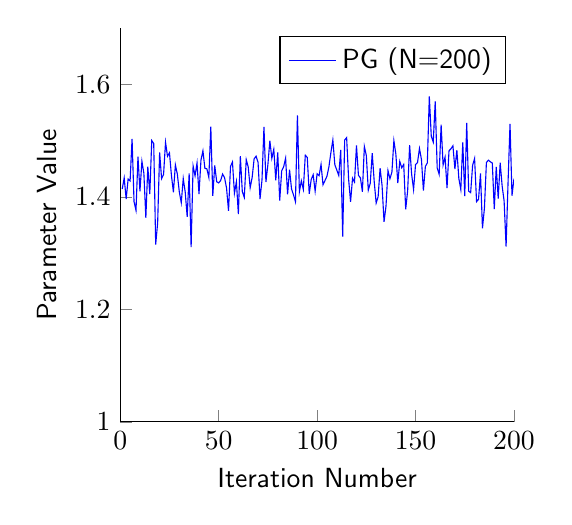
\begin{tikzpicture}

\begin{axis}[%
width=5cm,
height=5cm,
scale only axis,
xmin=0,
xmax=200,
xlabel={Iteration Number},
ymin=1,
ymax=1.7,
ylabel={Parameter Value},
axis x line*=bottom,
axis y line*=left,
legend style={draw=black,fill=white,legend cell align=left}
]
\addplot [
color=blue,
solid
]
table[row sep=crcr]{
1 1.4142135623731\\
2 1.43377352870439\\
3 1.3963131353002\\
4 1.43197842833625\\
5 1.42859687957848\\
6 1.50335600873405\\
7 1.39156082964571\\
8 1.37609043168337\\
9 1.47170665394612\\
10 1.40991000475012\\
11 1.46345003852921\\
12 1.44187313898492\\
13 1.36276416273975\\
14 1.45403706975163\\
15 1.4052933086616\\
16 1.50026618382828\\
17 1.49485375940985\\
18 1.31539694603256\\
19 1.35395607613299\\
20 1.4791216595247\\
21 1.43264462538736\\
22 1.43982160147583\\
23 1.49722900541711\\
24 1.47241113839952\\
25 1.47848574596163\\
26 1.43827872660358\\
27 1.40843107484716\\
28 1.45700548070351\\
29 1.44060656982749\\
30 1.40876632869546\\
31 1.38979446593542\\
32 1.43282978463968\\
33 1.40858990672707\\
34 1.36461205567222\\
35 1.44178662755907\\
36 1.31076310336797\\
37 1.45504303350344\\
38 1.43769018993522\\
39 1.46028053646831\\
40 1.40524121456355\\
41 1.46543838225841\\
42 1.48196136053121\\
43 1.45085380140558\\
44 1.45000820057836\\
45 1.43483878522219\\
46 1.52489857749719\\
47 1.40194606447565\\
48 1.45591631762581\\
49 1.42694438808307\\
50 1.42500822880822\\
51 1.42919937721888\\
52 1.44070259739459\\
53 1.43409202804979\\
54 1.41571877954808\\
55 1.37512983107634\\
56 1.45413719480114\\
57 1.46223328711744\\
58 1.40646314857432\\
59 1.42706953790859\\
60 1.36971732053334\\
61 1.47244878718287\\
62 1.40959757375437\\
63 1.39907031981812\\
64 1.46636052783259\\
65 1.45335933502549\\
66 1.41645071471736\\
67 1.43457770809791\\
68 1.46771180830121\\
69 1.47243436278692\\
70 1.46158313390464\\
71 1.39640918053649\\
72 1.43012154253543\\
73 1.52453407301103\\
74 1.42663665215189\\
75 1.45771495854355\\
76 1.49994610566943\\
77 1.46855509600684\\
78 1.48476008711824\\
79 1.4294009600944\\
80 1.47924175942086\\
81 1.39339316644951\\
82 1.44629496477867\\
83 1.45351039173426\\
84 1.46889269355782\\
85 1.40452186650759\\
86 1.44837599204574\\
87 1.41444959570685\\
88 1.40390583178979\\
89 1.39156567762127\\
90 1.54517355526581\\
91 1.40936579333009\\
92 1.42873596029867\\
93 1.41340310836546\\
94 1.4741455641649\\
95 1.47033467398831\\
96 1.40551737451868\\
97 1.43103490190875\\
98 1.43943661392148\\
99 1.41033414633683\\
100 1.44109063380287\\
101 1.43778730940363\\
102 1.45776580416018\\
103 1.42177110685696\\
104 1.4291942055182\\
105 1.43679003397294\\
106 1.45365027579586\\
107 1.47878734334729\\
108 1.50134326976209\\
109 1.45732426141861\\
110 1.44788888605762\\
111 1.43825963229144\\
112 1.48381863323553\\
113 1.32958217922754\\
114 1.50114503279375\\
115 1.50552927327944\\
116 1.43180514432739\\
117 1.39123574660834\\
118 1.43341991417257\\
119 1.4265080078318\\
120 1.49158148693198\\
121 1.43839439636457\\
122 1.43401142911837\\
123 1.40924965877397\\
124 1.48970196436626\\
125 1.47381798163989\\
126 1.41205777732321\\
127 1.42435155977587\\
128 1.47802174711335\\
129 1.42777863110474\\
130 1.38917801400537\\
131 1.40042271358228\\
132 1.45114639247075\\
133 1.42034744769769\\
134 1.35582393519264\\
135 1.38384474946508\\
136 1.44680322718019\\
137 1.43238676324923\\
138 1.44405117189515\\
139 1.5001622212527\\
140 1.47634852768802\\
141 1.42466857831078\\
142 1.46314230614712\\
143 1.45189416453364\\
144 1.45783226568481\\
145 1.37793365205478\\
146 1.41122290926889\\
147 1.49222568981485\\
148 1.44104819008748\\
149 1.41320124485468\\
150 1.45762498671507\\
151 1.46103189692245\\
152 1.48612147942153\\
153 1.46674232744054\\
154 1.41133848618699\\
155 1.45429357642735\\
156 1.46058994578566\\
157 1.57891079124933\\
158 1.50777585472434\\
159 1.49738888487944\\
160 1.5698717174439\\
161 1.45163932009063\\
162 1.44029211923803\\
163 1.52843266369763\\
164 1.45693547947378\\
165 1.47065629652682\\
166 1.41586778335086\\
167 1.48202888565075\\
168 1.4857154841912\\
169 1.49091077182315\\
170 1.44964133620201\\
171 1.4832006883655\\
172 1.43268483093865\\
173 1.41320624214677\\
174 1.49697258680448\\
175 1.40169579768688\\
176 1.53157177460985\\
177 1.41025949533653\\
178 1.40763306320119\\
179 1.45639232890202\\
180 1.46838750793705\\
181 1.39161654917694\\
182 1.39567891043664\\
183 1.44182702098288\\
184 1.34403367901962\\
185 1.38028768124853\\
186 1.46127483178683\\
187 1.46535324265971\\
188 1.46265429996712\\
189 1.46017789576406\\
190 1.37826491377238\\
191 1.4535427460602\\
192 1.39729164168621\\
193 1.46076624802539\\
194 1.41939824474309\\
195 1.39282256676631\\
196 1.3115662474662\\
197 1.42587783840001\\
198 1.52990994906988\\
199 1.4022381744742\\
200 1.43232584740283\\
};
\addlegendentry{PG (N=200)};

\addplot [
color=black,
dotted,
forget plot
]
table[row sep=crcr]{
1 1\\
200 1\\
};
\end{axis}
\end{tikzpicture}%
\caption{First 200 iterations using PG with 200 particles. Chain fails to converge at all, even after 5000 iterations.}
\label{fig:chain_init_fail}
\end{figure}

\begin{figure}
\centering
% This file was created by matlab2tikz v0.4.4 running on MATLAB 7.13.
% Copyright (c) 2008--2013, Nico Schlömer <nico.schloemer@gmail.com>
% All rights reserved.
% 
% The latest updates can be retrieved from
%   http://www.mathworks.com/matlabcentral/fileexchange/22022-matlab2tikz
% where you can also make suggestions and rate matlab2tikz.
% 
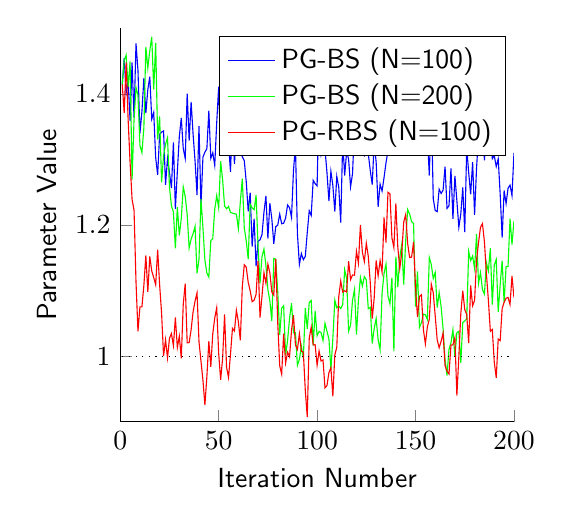
\begin{tikzpicture}

\begin{axis}[%
width=5cm,
height=5cm,
scale only axis,
xmin=0,
xmax=200,
xlabel={Iteration Number},
ymin=0.9,
ymax=1.5,
ylabel={Parameter Value},
axis x line*=bottom,
axis y line*=left,
legend style={draw=black,fill=white,legend cell align=left}
]
\addplot [
color=blue,
solid
]
table[row sep=crcr]{
1 1.4142135623731\\
2 1.45481860160839\\
3 1.40158491372388\\
4 1.42063709957098\\
5 1.35853429984468\\
6 1.44793765288687\\
7 1.36368198723882\\
8 1.47676631571407\\
9 1.43589505943837\\
10 1.33992235234357\\
11 1.37280585677563\\
12 1.42421378712093\\
13 1.37052412868845\\
14 1.40629295812517\\
15 1.42615614219332\\
16 1.36144622462903\\
17 1.37170483485169\\
18 1.30282122576373\\
19 1.27652881392504\\
20 1.33836335451441\\
21 1.34160781088656\\
22 1.34349500312676\\
23 1.26114338405133\\
24 1.30156951834672\\
25 1.280052314584\\
26 1.25622801123156\\
27 1.32593097718461\\
28 1.2246489951094\\
29 1.28132573854091\\
30 1.33470377230278\\
31 1.36331552714548\\
32 1.31685852591451\\
33 1.30152911223469\\
34 1.40029571502055\\
35 1.32870235838645\\
36 1.38760685614\\
37 1.33832531634842\\
38 1.29763536590727\\
39 1.24585091002248\\
40 1.35093671942394\\
41 1.22911509052124\\
42 1.30347937840859\\
43 1.31112854417968\\
44 1.31629825932518\\
45 1.37419532663224\\
46 1.30171809211506\\
47 1.31016876625092\\
48 1.29101192578097\\
49 1.35600602825814\\
50 1.41079190628558\\
51 1.3214295303662\\
52 1.34969595533729\\
53 1.3654398253292\\
54 1.33213739095462\\
55 1.3239429530921\\
56 1.28103045618515\\
57 1.36627635288689\\
58 1.29319304860341\\
59 1.34028719331486\\
60 1.40239817781173\\
61 1.31900154047798\\
62 1.30430046053707\\
63 1.29802883081675\\
64 1.26612430655181\\
65 1.22108212249412\\
66 1.249382000956\\
67 1.16703610548762\\
68 1.20965641750402\\
69 1.13730141854502\\
70 1.17527215969231\\
71 1.17746333150401\\
72 1.18529888758378\\
73 1.21955482752741\\
74 1.24445491355219\\
75 1.17953530801645\\
76 1.23322457091445\\
77 1.20942974642963\\
78 1.17159350902278\\
79 1.19754665684774\\
80 1.19993934015537\\
81 1.21673214204855\\
82 1.20203015049748\\
83 1.20279439415426\\
84 1.21072170107316\\
85 1.23060168736068\\
86 1.22647015901679\\
87 1.2117094648394\\
88 1.28343248056427\\
89 1.32036458119113\\
90 1.18676299912278\\
91 1.13997126749305\\
92 1.15658842670357\\
93 1.14722198863084\\
94 1.15237828872079\\
95 1.18860073649533\\
96 1.22178502441518\\
97 1.21463258901981\\
98 1.26826198742325\\
99 1.26324418239997\\
100 1.25970310758068\\
101 1.3925764385402\\
102 1.30653777882698\\
103 1.31529794610675\\
104 1.31562884541656\\
105 1.28042395003456\\
106 1.23664884666128\\
107 1.28195476735073\\
108 1.2604826738157\\
109 1.22072601632386\\
110 1.27423104066005\\
111 1.25744404083678\\
112 1.20365332111912\\
113 1.32697081555274\\
114 1.27552152230887\\
115 1.31181493060896\\
116 1.300321751254\\
117 1.25838254448155\\
118 1.27839707563806\\
119 1.3521182524339\\
120 1.3546679896425\\
121 1.37845725884672\\
122 1.34259525889199\\
123 1.3751041281137\\
124 1.30427233577804\\
125 1.36476014765708\\
126 1.3089256328933\\
127 1.28327481887199\\
128 1.26187327088228\\
129 1.32652277488323\\
130 1.2954762542599\\
131 1.22793675233294\\
132 1.26226904894296\\
133 1.25185025417374\\
134 1.27231427432875\\
135 1.29493259790254\\
136 1.31296317424523\\
137 1.37568374623567\\
138 1.43707520316721\\
139 1.43130179881485\\
140 1.38241082848777\\
141 1.38394232207953\\
142 1.31358342609755\\
143 1.39414699239155\\
144 1.38504676641152\\
145 1.4410892183421\\
146 1.48199274575989\\
147 1.35911477373942\\
148 1.36346564768127\\
149 1.32553625541457\\
150 1.3433823543142\\
151 1.37453507875475\\
152 1.36756186079229\\
153 1.33029865421786\\
154 1.32627510337857\\
155 1.32953932568467\\
156 1.33597852029979\\
157 1.27558223139805\\
158 1.38431159112569\\
159 1.24005146218849\\
160 1.22210993727263\\
161 1.22049029016608\\
162 1.25466505198034\\
163 1.24816523076658\\
164 1.25321372706576\\
165 1.28915127714532\\
166 1.22538375415465\\
167 1.22942010348294\\
168 1.2863200318166\\
169 1.20961164505158\\
170 1.27506298842779\\
171 1.23712463452053\\
172 1.19665193192088\\
173 1.21710456864523\\
174 1.25739717411954\\
175 1.18929527453161\\
176 1.31712047672716\\
177 1.28010242410244\\
178 1.24694609434587\\
179 1.29597646207732\\
180 1.2156133307405\\
181 1.28701025768881\\
182 1.33704250832473\\
183 1.3366644908864\\
184 1.36282117424182\\
185 1.29850790553231\\
186 1.34401527013884\\
187 1.38994426929179\\
188 1.39300968788342\\
189 1.30111941358276\\
190 1.30579876607791\\
191 1.28917983086101\\
192 1.3010963388943\\
193 1.24691754331651\\
194 1.18095518411793\\
195 1.25265548734682\\
196 1.23275873133612\\
197 1.25624207707393\\
198 1.26088202714202\\
199 1.24497869958662\\
200 1.30999087071671\\
};
\addlegendentry{PG-BS (N=100)};

\addplot [
color=green,
solid
]
table[row sep=crcr]{
1 1.4142135623731\\
2 1.45022086324922\\
3 1.45915661506643\\
4 1.41018559375724\\
5 1.44944827758191\\
6 1.26934568319974\\
7 1.36056944251801\\
8 1.40964409452772\\
9 1.39817305235935\\
10 1.32099927786595\\
11 1.31052345648389\\
12 1.34840568251384\\
13 1.47158601640702\\
14 1.43932974277776\\
15 1.46570686885645\\
16 1.48685161864869\\
17 1.40697845905602\\
18 1.47761024469544\\
19 1.33047823869567\\
20 1.36546960515894\\
21 1.26519786771801\\
22 1.30560352180377\\
23 1.32302362233972\\
24 1.33312957745395\\
25 1.25758542897383\\
26 1.22929345901731\\
27 1.22006689545157\\
28 1.16452011519571\\
29 1.2273731140404\\
30 1.18430794763316\\
31 1.21004241194693\\
32 1.25820886162625\\
33 1.24360039694981\\
34 1.21603563982365\\
35 1.1648903073865\\
36 1.17869374903259\\
37 1.18684089353925\\
38 1.19810110542215\\
39 1.12649005215001\\
40 1.14792176985548\\
41 1.23991579322651\\
42 1.1962648139841\\
43 1.14662374459774\\
44 1.12686326025087\\
45 1.12081956770605\\
46 1.17647537560499\\
47 1.17953507573211\\
48 1.22407911210675\\
49 1.24498659519191\\
50 1.22626427142722\\
51 1.2975285284802\\
52 1.26884305122215\\
53 1.22900566659355\\
54 1.22489355274749\\
55 1.22828469799697\\
56 1.21936851704531\\
57 1.21822215698031\\
58 1.21732076613048\\
59 1.21655110991132\\
60 1.19466965734699\\
61 1.23566017530089\\
62 1.27074312948403\\
63 1.19578129864211\\
64 1.17578786436414\\
65 1.14833241806529\\
66 1.23197817473419\\
67 1.2261576896121\\
68 1.22348770188639\\
69 1.2457094284329\\
70 1.16783122763494\\
71 1.11116576688667\\
72 1.15189758934353\\
73 1.16351649702424\\
74 1.13810480620598\\
75 1.10141689893568\\
76 1.08466109281531\\
77 1.05385668757456\\
78 1.14927122515633\\
79 1.14789771458247\\
80 1.09848159052436\\
81 1.03263809155181\\
82 1.07348901193274\\
83 1.07718354937112\\
84 1.00158204233649\\
85 1.02426240180712\\
86 1.0578689543223\\
87 1.08102731815762\\
88 1.03596061358248\\
89 1.03585493087932\\
90 0.986305840148676\\
91 0.995431360851552\\
92 1.01546436343573\\
93 0.996714245236989\\
94 1.07354430292528\\
95 1.04190693780048\\
96 1.08189346484734\\
97 1.08514582641078\\
98 1.01647287701822\\
99 1.06903339212887\\
100 1.0315059330456\\
101 1.03803447787689\\
102 1.03624418129696\\
103 1.02410244142132\\
104 1.05024271188435\\
105 1.03823524110259\\
106 1.02657507702424\\
107 0.980250628590709\\
108 1.02748644814341\\
109 1.08548720008392\\
110 1.073913726615\\
111 1.07680824282292\\
112 1.0727330140584\\
113 1.07870506104706\\
114 1.13213117186429\\
115 1.11857369847474\\
116 1.03835492059489\\
117 1.04743843480806\\
118 1.08562509078516\\
119 1.10218335635798\\
120 1.03298563821147\\
121 1.08556573026256\\
122 1.12028099125154\\
123 1.10692031897134\\
124 1.12137703128794\\
125 1.11646911229014\\
126 1.07258065938998\\
127 1.07464599324131\\
128 1.01963169661351\\
129 1.04225264801581\\
130 1.05749729597529\\
131 1.02499243162532\\
132 1.01033727387601\\
133 1.09610634087796\\
134 1.12619821238448\\
135 1.14044953599726\\
136 1.0917800441768\\
137 1.07993089438954\\
138 1.11991734461291\\
139 1.00791095462946\\
140 1.15185224410682\\
141 1.1056327351102\\
142 1.15107769971522\\
143 1.17027809632949\\
144 1.10937878599026\\
145 1.17645305623651\\
146 1.22351480667838\\
147 1.21687581500948\\
148 1.20518605738662\\
149 1.20239529552098\\
150 1.07587385773864\\
151 1.12921058544214\\
152 1.04398891697433\\
153 1.05150469347712\\
154 1.06434814512845\\
155 1.0631148523934\\
156 1.05616150114751\\
157 1.15073331633856\\
158 1.13993723410926\\
159 1.11853196783262\\
160 1.12784858657962\\
161 1.07425281692344\\
162 1.09722171736581\\
163 1.07561322586228\\
164 1.04166311570637\\
165 0.99441316217143\\
166 0.970616951276475\\
167 1.01095645969466\\
168 1.02053891381914\\
169 1.04063287424992\\
170 0.999147264673727\\
171 1.03615754207839\\
172 1.03814073244633\\
173 0.990119148410322\\
174 1.05132982707764\\
175 1.05403697391652\\
176 1.0567876554409\\
177 1.15982365049603\\
178 1.14599773119081\\
179 1.15290891473697\\
180 1.13373512976453\\
181 1.18633186256715\\
182 1.11089181777351\\
183 1.12772944113563\\
184 1.10160785331031\\
185 1.09468104684394\\
186 1.14268016143274\\
187 1.12977947190618\\
188 1.16474943612889\\
189 1.0788911949522\\
190 1.13891799211552\\
191 1.14772655670331\\
192 1.06789929564016\\
193 1.10901925297473\\
194 1.14579527387063\\
195 1.08174499614245\\
196 1.13706304202515\\
197 1.13669276598724\\
198 1.20967163560992\\
199 1.17035891772787\\
200 1.2061926305546\\
};
\addlegendentry{PG-BS (N=200)};

\addplot [
color=red,
solid
]
table[row sep=crcr]{
1 1.4142135623731\\
2 1.37119703356863\\
3 1.44775991497822\\
4 1.36064220106031\\
5 1.29492338469448\\
6 1.23918985629225\\
7 1.22281171417818\\
8 1.11333590088372\\
9 1.03804051611369\\
10 1.07539354849837\\
11 1.07526064427694\\
12 1.10802350697278\\
13 1.15362941202431\\
14 1.09812641708343\\
15 1.15221596185733\\
16 1.13012298690016\\
17 1.11995445075836\\
18 1.10897471800386\\
19 1.1624012275137\\
20 1.10909312985712\\
21 1.06561246105403\\
22 1.00054895141117\\
23 1.02532437628957\\
24 0.997565129965696\\
25 1.0273307608967\\
26 1.03469053187397\\
27 1.01620205103953\\
28 1.05933936722339\\
29 1.01351651059155\\
30 1.03054216132972\\
31 0.996822274325872\\
32 1.07939059502006\\
33 1.11080611892695\\
34 1.02061685330744\\
35 1.0208985787014\\
36 1.04049556571632\\
37 1.06791536599834\\
38 1.0842385830762\\
39 1.09679152673722\\
40 1.02224957874212\\
41 0.992724794837034\\
42 0.963907002945354\\
43 0.925684073745338\\
44 0.96879749630044\\
45 1.02314131013817\\
46 0.98394551392845\\
47 1.03463694048203\\
48 1.05828784009005\\
49 1.0741107631112\\
50 1.00438571792938\\
51 0.964133651043562\\
52 0.997063439157196\\
53 1.06375208367906\\
54 0.983583171851757\\
55 0.967722121180636\\
56 1.00318543746288\\
57 1.0426316486993\\
58 1.03851197876087\\
59 1.07004527671633\\
60 1.05286616966882\\
61 1.0243213887998\\
62 1.10626673787544\\
63 1.13954858458267\\
64 1.13572110144321\\
65 1.11264709270763\\
66 1.09984084328057\\
67 1.08330295270485\\
68 1.08553922950855\\
69 1.09432401345422\\
70 1.1448674467437\\
71 1.05909784139051\\
72 1.09150228431621\\
73 1.12733040299771\\
74 1.11150391941635\\
75 1.1403995372275\\
76 1.12739469560286\\
77 1.09770794435088\\
78 1.09318892920069\\
79 1.14838091940078\\
80 1.05060657444828\\
81 0.985677099824565\\
82 0.972710301940158\\
83 1.03433829322793\\
84 0.989828035096941\\
85 1.00615006447708\\
86 0.999427819538049\\
87 1.03943611340475\\
88 1.06268173456841\\
89 1.01717805322163\\
90 1.01045982522409\\
91 1.03428865131061\\
92 1.00764644183801\\
93 1.00646291882503\\
94 0.948079800626466\\
95 0.907430476233188\\
96 1.02748869138715\\
97 1.04427525461978\\
98 1.01742121155543\\
99 1.01760763612543\\
100 0.986472027855865\\
101 1.00807339226522\\
102 0.992731342732307\\
103 0.994441461230235\\
104 0.951874437754507\\
105 0.955354573763725\\
106 0.975054067383037\\
107 0.982654915778683\\
108 0.93899162941958\\
109 1.0021123665563\\
110 1.01385481789094\\
111 1.09076871845848\\
112 1.11491073495572\\
113 1.09786543488758\\
114 1.09990661435362\\
115 1.09805691175427\\
116 1.14485624844136\\
117 1.11704046889894\\
118 1.12400747304842\\
119 1.1236120430789\\
120 1.1600316256432\\
121 1.1419427809347\\
122 1.20037687462522\\
123 1.15846687784975\\
124 1.1445051343627\\
125 1.17220610549887\\
126 1.15238096965612\\
127 1.11256249928779\\
128 1.05736942429618\\
129 1.08883530862029\\
130 1.14622992948415\\
131 1.12259687145333\\
132 1.14590263971859\\
133 1.12836549012591\\
134 1.21175869221712\\
135 1.17340985838348\\
136 1.24987485015186\\
137 1.24761516463469\\
138 1.18061787601622\\
139 1.16593683955981\\
140 1.23290185121087\\
141 1.1661447182299\\
142 1.13396215533918\\
143 1.15782696751106\\
144 1.20449455678083\\
145 1.21603560111021\\
146 1.1717348952268\\
147 1.15045327335245\\
148 1.15119004505194\\
149 1.17429886468404\\
150 1.10444539458793\\
151 1.05965187462955\\
152 1.09122251065256\\
153 1.09383772990472\\
154 1.0404792778542\\
155 1.01882110539118\\
156 1.04463694922995\\
157 1.05663314649066\\
158 1.11002054102321\\
159 1.09682757806305\\
160 1.06149277474879\\
161 1.02524384421852\\
162 1.01300457840946\\
163 1.02307616636574\\
164 1.03535741494004\\
165 0.985612579618806\\
166 0.977301924585859\\
167 0.973104371918905\\
168 1.01706088116277\\
169 1.01743814224657\\
170 1.02860488223425\\
171 0.940055243789263\\
172 0.999438803983715\\
173 1.06491727836319\\
174 1.09983897348975\\
175 1.07126725634134\\
176 1.06369888003304\\
177 1.02003266546872\\
178 1.10795915096442\\
179 1.0769814724693\\
180 1.08521432411089\\
181 1.14671606896523\\
182 1.17309101200442\\
183 1.19671566634952\\
184 1.20219594632451\\
185 1.17440242801876\\
186 1.1258299843661\\
187 1.08594021540099\\
188 1.03821339234467\\
189 1.0408248774775\\
190 0.991118162878846\\
191 0.96718805366098\\
192 1.02623000029966\\
193 1.02393334658338\\
194 1.07283085119296\\
195 1.08226733422479\\
196 1.08858697770104\\
197 1.08966866405069\\
198 1.07892423741731\\
199 1.12238247958536\\
200 1.08948605248465\\
};
\addlegendentry{PG-RBS (N=100)};

\addplot [
color=black,
dotted,
forget plot
]
table[row sep=crcr]{
1 1\\
200 1\\
};
\end{axis}
\end{tikzpicture}%
\caption{First 200 iterations using PG-BS and PG-RBS. Faster convergence with PG-RBS.}
\label{fig:chain_init}
\end{figure}

\begin{figure}
\centering
% This file was created by matlab2tikz v0.4.4 running on MATLAB 7.13.
% Copyright (c) 2008--2013, Nico Schlömer <nico.schloemer@gmail.com>
% All rights reserved.
% 
% The latest updates can be retrieved from
%   http://www.mathworks.com/matlabcentral/fileexchange/22022-matlab2tikz
% where you can also make suggestions and rate matlab2tikz.
% 
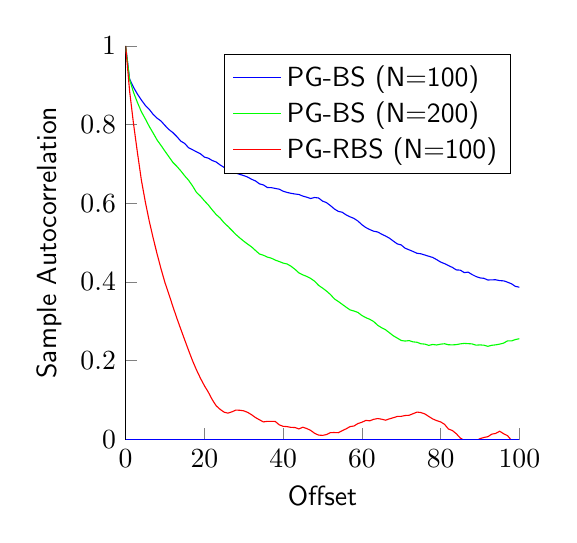
\begin{tikzpicture}

\begin{axis}[%
width=5cm,
height=5cm,
scale only axis,
xmin=0,
xmax=100,
xlabel={Offset},
ymin=0,
ymax=1,
ylabel={Sample Autocorrelation},
axis x line*=bottom,
axis y line*=left,
legend style={draw=black,fill=white,legend cell align=left}
]
\addplot [
color=blue,
solid
]
table[row sep=crcr]{
0 0.999798281312059\\
1 0.915624121112439\\
2 0.894776311954964\\
3 0.877216911027432\\
4 0.862246682145831\\
5 0.848743641657417\\
6 0.838692155669459\\
7 0.825695164625249\\
8 0.816175022730327\\
9 0.808821733875103\\
10 0.797552430208437\\
11 0.787301722874029\\
12 0.779513341604263\\
13 0.769409876064295\\
14 0.758022506952182\\
15 0.752050004835899\\
16 0.740936382236225\\
17 0.735942538342127\\
18 0.730871230352638\\
19 0.725799496296792\\
20 0.717356046081224\\
21 0.71455857748868\\
22 0.70869850798143\\
23 0.704840005011705\\
24 0.697363899669201\\
25 0.691293148389707\\
26 0.685349393231055\\
27 0.683594773361235\\
28 0.676641929354731\\
29 0.673415811964474\\
30 0.670397728687931\\
31 0.666553098607651\\
32 0.661050328945236\\
33 0.656679998630845\\
34 0.649350805092292\\
35 0.646582753421828\\
36 0.640060563274017\\
37 0.639805147013295\\
38 0.63775472851185\\
39 0.635822867829615\\
40 0.630704425107676\\
41 0.62764206462701\\
42 0.625344411805786\\
43 0.623623979384397\\
44 0.622370494524757\\
45 0.618331540550863\\
46 0.615536123028028\\
47 0.612232433686233\\
48 0.614755082305426\\
49 0.613474896429257\\
50 0.605691018475423\\
51 0.601744331901164\\
52 0.594304290686733\\
53 0.585800916997999\\
54 0.579489125303258\\
55 0.577284853831958\\
56 0.570696900769911\\
57 0.565659299341635\\
58 0.561599037537632\\
59 0.554951305735708\\
60 0.54568751197232\\
61 0.53847467491627\\
62 0.533369874796613\\
63 0.529091368386307\\
64 0.527184236554971\\
65 0.521802538626919\\
66 0.516971722638917\\
67 0.511372503092128\\
68 0.504018690264989\\
69 0.496797611572603\\
70 0.494206532412249\\
71 0.485792863071703\\
72 0.481785599206563\\
73 0.477617501525361\\
74 0.473066879129099\\
75 0.471704592641023\\
76 0.468631691925583\\
77 0.465482323886108\\
78 0.46241503793514\\
79 0.456910663345093\\
80 0.450741956256203\\
81 0.446775694791504\\
82 0.441789313501472\\
83 0.437098023949077\\
84 0.430741539153932\\
85 0.430246535833283\\
86 0.423981567294983\\
87 0.425136344330151\\
88 0.419004670279828\\
89 0.414014137297297\\
90 0.41048670479262\\
91 0.409446710426441\\
92 0.405132026101865\\
93 0.40558853762261\\
94 0.405749827268178\\
95 0.403626336476277\\
96 0.402987028507362\\
97 0.399637083438771\\
98 0.39553156126548\\
99 0.389008512939281\\
100 0.386845189453636\\
};
\addlegendentry{PG-BS (N=100)};

\addplot [
color=green,
solid
]
table[row sep=crcr]{
0 0.999735668441313\\
1 0.914481181123425\\
2 0.881931384546857\\
3 0.855958992210686\\
4 0.832507787474133\\
5 0.814378364857554\\
6 0.795208619457232\\
7 0.778235168115491\\
8 0.760627796122512\\
9 0.746788892442977\\
10 0.732171392440284\\
11 0.718149867528279\\
12 0.703930891262658\\
13 0.693896218721349\\
14 0.682416169271748\\
15 0.669765143416776\\
16 0.658420934234354\\
17 0.644070867053783\\
18 0.627636183983486\\
19 0.618091119201831\\
20 0.606408296270717\\
21 0.595789701811203\\
22 0.58321185647807\\
23 0.571402038418741\\
24 0.562479259669943\\
25 0.550555047644616\\
26 0.541160119030734\\
27 0.531077984763337\\
28 0.520806256044741\\
29 0.511967129695123\\
30 0.503744723696589\\
31 0.496249956906597\\
32 0.489163504863905\\
33 0.480034900971962\\
34 0.471202638969409\\
35 0.46803863081975\\
36 0.463352655942135\\
37 0.460631919720581\\
38 0.455728385027552\\
39 0.452133278145331\\
40 0.448117728144302\\
41 0.445878623313912\\
42 0.440153760374035\\
43 0.43251857489461\\
44 0.423311824223957\\
45 0.418213476822314\\
46 0.414251670977437\\
47 0.409094391026042\\
48 0.402109792882777\\
49 0.391629562153667\\
50 0.384737321779958\\
51 0.377214451295985\\
52 0.368527600107138\\
53 0.357461624808768\\
54 0.350709200038253\\
55 0.343481792811383\\
56 0.336168696073733\\
57 0.329279236726287\\
58 0.326327040140531\\
59 0.322820048281983\\
60 0.315037099336333\\
61 0.309529013713906\\
62 0.30534373927285\\
63 0.299731397314584\\
64 0.290269220765721\\
65 0.284063305608856\\
66 0.278880878428492\\
67 0.271198283113526\\
68 0.263385111366395\\
69 0.257615940887156\\
70 0.251593270166341\\
71 0.250049029253574\\
72 0.251260769259554\\
73 0.248055081180055\\
74 0.247019409096633\\
75 0.2432212085562\\
76 0.242323271951378\\
77 0.239136090474182\\
78 0.241389225872058\\
79 0.240134957094162\\
80 0.24221178129875\\
81 0.243206899519972\\
82 0.240705085826255\\
83 0.240383814526176\\
84 0.241007518727542\\
85 0.242941326029456\\
86 0.24415615968832\\
87 0.243480309945566\\
88 0.242863767634756\\
89 0.239636451658059\\
90 0.24031881863746\\
91 0.239545795052911\\
92 0.236688134462873\\
93 0.2393804528265\\
94 0.24041379030899\\
95 0.242298822080309\\
96 0.244862693661909\\
97 0.250628352470316\\
98 0.250377643059829\\
99 0.253886461674362\\
100 0.256069918130852\\
};
\addlegendentry{PG-BS (N=200)};

\addplot [
color=red,
solid
]
table[row sep=crcr]{
0 0.999968823634988\\
1 0.885718646815701\\
2 0.802259863457898\\
3 0.728420964444668\\
4 0.658796851721707\\
5 0.603636929108635\\
6 0.554684036866382\\
7 0.511341314922726\\
8 0.470975574281194\\
9 0.433128732751877\\
10 0.398096402060836\\
11 0.368596893728835\\
12 0.337821490196935\\
13 0.308473972418703\\
14 0.280536468643352\\
15 0.253124398685446\\
16 0.226053846321716\\
17 0.199975633696805\\
18 0.176706793928927\\
19 0.155632632637222\\
20 0.136814922247788\\
21 0.120272628857837\\
22 0.101149960397839\\
23 0.0856885874961511\\
24 0.0766596706175781\\
25 0.0695169076861798\\
26 0.0669462337183461\\
27 0.0702814312296625\\
28 0.0748199267353808\\
29 0.0742932389146709\\
30 0.0728580835705744\\
31 0.0689101431494078\\
32 0.0628727157913182\\
33 0.0556759987492903\\
34 0.050029273044803\\
35 0.0446431255860951\\
36 0.0462549718248574\\
37 0.0459265104860805\\
38 0.0458928046222011\\
39 0.0374328522499704\\
40 0.0334899385238281\\
41 0.03282445492212\\
42 0.030754101785303\\
43 0.0305848965993576\\
44 0.0269034309731672\\
45 0.0311715882292827\\
46 0.0279195100695634\\
47 0.0231290826015838\\
48 0.0158584988791943\\
49 0.0112250598448218\\
50 0.0105440545001774\\
51 0.012486996794165\\
52 0.0175629465227167\\
53 0.0177334781672981\\
54 0.0173073996379803\\
55 0.0224664413047218\\
56 0.0271237730041279\\
57 0.0327795919209489\\
58 0.0343445992493485\\
59 0.0406237395754402\\
60 0.0437594951784934\\
61 0.0485713220842994\\
62 0.0475398750833515\\
63 0.0512796579575216\\
64 0.0532637592804504\\
65 0.0517495565556907\\
66 0.0491075852126333\\
67 0.0524874398796972\\
68 0.0553814644665979\\
69 0.0585984910610253\\
70 0.0588765842698647\\
71 0.0609902341618591\\
72 0.0615823550027252\\
73 0.0654990392420153\\
74 0.0696699371336951\\
75 0.0684665591810113\\
76 0.0649792097944126\\
77 0.0585444875947864\\
78 0.0523297552300592\\
79 0.0479626114359888\\
80 0.0447828267133054\\
81 0.0385991829493327\\
82 0.0265991517077248\\
83 0.0228245468497075\\
84 0.0146316268590258\\
85 0.00371475791139931\\
86 -0.00193069042068994\\
87 -0.00508647340766853\\
88 -0.00634094246486448\\
89 -0.00316688666572656\\
90 0.00220759955810218\\
91 0.00514869054228073\\
92 0.0072361679978563\\
93 0.0135785579907695\\
94 0.0155350152867263\\
95 0.0209717224626127\\
96 0.0147975353741198\\
97 0.00984982534527234\\
98 -0.00192268956700013\\
99 -0.0110744286805041\\
100 -0.0166916896123809\\
};
\addlegendentry{PG-RBS (N=100)};

\addplot [
color=blue,
solid,
forget plot
]
table[row sep=crcr]{
0 0\\
100 0\\
};
\end{axis}
\end{tikzpicture}%
\caption{Autocorrelation plot for PG-BS and PG-RBS.}
\label{fig:acf}
\end{figure}

\begin{figure}
\centering
\subfloat[PG-BS (N=100)]{ % This file was created by matlab2tikz v0.4.4 running on MATLAB 7.13.
% Copyright (c) 2008--2013, Nico Schlömer <nico.schloemer@gmail.com>
% All rights reserved.
% 
% The latest updates can be retrieved from
%   http://www.mathworks.com/matlabcentral/fileexchange/22022-matlab2tikz
% where you can also make suggestions and rate matlab2tikz.
% 
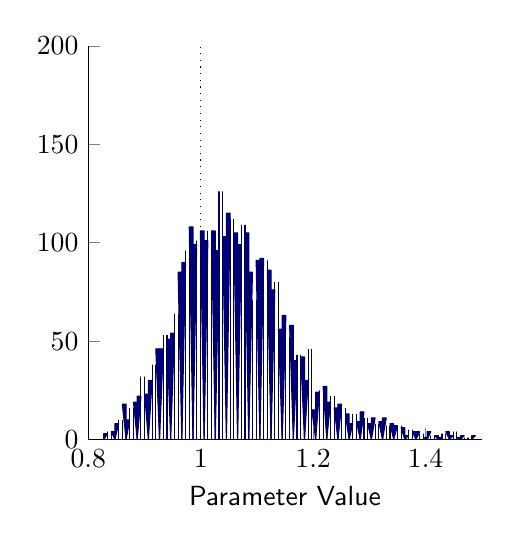
\begin{tikzpicture}

\begin{axis}[%
width=5cm,
height=5cm,
colormap/jet,
scale only axis,
xmin=0.8,
xmax=1.5,
xlabel={Parameter Value},
ymin=0,
ymax=200,
axis x line*=bottom,
axis y line*=left
]

\addplot[area legend,patch,forget plot]
table[row sep=crcr, point meta=\thisrow{c}]{
x y c\\
0.827707248117718 0 1 \\
0.827707248117718 3 1 \\
0.834315958171122 3 1 \\
0.834315958171122 0 1 \\
0.834315958171122 0 1 \\
0.834315958171122 4 1 \\
0.840924668224526 4 1 \\
0.840924668224526 0 1 \\
0.840924668224527 0 1 \\
0.840924668224527 4 1 \\
0.847533378277931 4 1 \\
0.847533378277931 0 1 \\
0.847533378277931 0 1 \\
0.847533378277931 8 1 \\
0.854142088331335 8 1 \\
0.854142088331335 0 1 \\
0.854142088331335 0 1 \\
0.854142088331335 10 1 \\
0.86075079838474 10 1 \\
0.86075079838474 0 1 \\
0.86075079838474 0 1 \\
0.86075079838474 18 1 \\
0.867359508438144 18 1 \\
0.867359508438144 0 1 \\
0.867359508438144 0 1 \\
0.867359508438144 10 1 \\
0.873968218491548 10 1 \\
0.873968218491548 0 1 \\
0.873968218491548 0 1 \\
0.873968218491548 16 1 \\
0.880576928544953 16 1 \\
0.880576928544953 0 1 \\
0.880576928544953 0 1 \\
0.880576928544953 19 1 \\
0.887185638598357 19 1 \\
0.887185638598357 0 1 \\
0.887185638598357 0 1 \\
0.887185638598357 22 1 \\
0.893794348651762 22 1 \\
0.893794348651762 0 1 \\
0.893794348651762 0 1 \\
0.893794348651762 32 1 \\
0.900403058705166 32 1 \\
0.900403058705166 0 1 \\
0.900403058705166 0 1 \\
0.900403058705166 23 1 \\
0.90701176875857 23 1 \\
0.90701176875857 0 1 \\
0.90701176875857 0 1 \\
0.90701176875857 30 1 \\
0.913620478811975 30 1 \\
0.913620478811975 0 1 \\
0.913620478811975 0 1 \\
0.913620478811975 38 1 \\
0.920229188865379 38 1 \\
0.920229188865379 0 1 \\
0.920229188865379 0 1 \\
0.920229188865379 46 1 \\
0.926837898918783 46 1 \\
0.926837898918783 0 1 \\
0.926837898918784 0 1 \\
0.926837898918784 46 1 \\
0.933446608972188 46 1 \\
0.933446608972188 0 1 \\
0.933446608972188 0 1 \\
0.933446608972188 53 1 \\
0.940055319025592 53 1 \\
0.940055319025592 0 1 \\
0.940055319025592 0 1 \\
0.940055319025592 51 1 \\
0.946664029078997 51 1 \\
0.946664029078997 0 1 \\
0.946664029078997 0 1 \\
0.946664029078997 54 1 \\
0.953272739132401 54 1 \\
0.953272739132401 0 1 \\
0.953272739132401 0 1 \\
0.953272739132401 64 1 \\
0.959881449185805 64 1 \\
0.959881449185805 0 1 \\
0.959881449185805 0 1 \\
0.959881449185805 85 1 \\
0.96649015923921 85 1 \\
0.96649015923921 0 1 \\
0.96649015923921 0 1 \\
0.96649015923921 90 1 \\
0.973098869292614 90 1 \\
0.973098869292614 0 1 \\
0.973098869292614 0 1 \\
0.973098869292614 96 1 \\
0.979707579346018 96 1 \\
0.979707579346018 0 1 \\
0.979707579346019 0 1 \\
0.979707579346019 108 1 \\
0.986316289399423 108 1 \\
0.986316289399423 0 1 \\
0.986316289399423 0 1 \\
0.986316289399423 99 1 \\
0.992924999452827 99 1 \\
0.992924999452827 0 1 \\
0.992924999452827 0 1 \\
0.992924999452827 101 1 \\
0.999533709506232 101 1 \\
0.999533709506232 0 1 \\
0.999533709506232 0 1 \\
0.999533709506232 106 1 \\
1.00614241955964 106 1 \\
1.00614241955964 0 1 \\
1.00614241955964 0 1 \\
1.00614241955964 101 1 \\
1.01275112961304 101 1 \\
1.01275112961304 0 1 \\
1.01275112961304 0 1 \\
1.01275112961304 106 1 \\
1.01935983966644 106 1 \\
1.01935983966644 0 1 \\
1.01935983966644 0 1 \\
1.01935983966644 106 1 \\
1.02596854971985 106 1 \\
1.02596854971985 0 1 \\
1.02596854971985 0 1 \\
1.02596854971985 96 1 \\
1.03257725977325 96 1 \\
1.03257725977325 0 1 \\
1.03257725977325 0 1 \\
1.03257725977325 126 1 \\
1.03918596982666 126 1 \\
1.03918596982666 0 1 \\
1.03918596982666 0 1 \\
1.03918596982666 103 1 \\
1.04579467988006 103 1 \\
1.04579467988006 0 1 \\
1.04579467988006 0 1 \\
1.04579467988006 115 1 \\
1.05240338993347 115 1 \\
1.05240338993347 0 1 \\
1.05240338993347 0 1 \\
1.05240338993347 112 1 \\
1.05901209998687 112 1 \\
1.05901209998687 0 1 \\
1.05901209998687 0 1 \\
1.05901209998687 105 1 \\
1.06562081004028 105 1 \\
1.06562081004028 0 1 \\
1.06562081004028 0 1 \\
1.06562081004028 99 1 \\
1.07222952009368 99 1 \\
1.07222952009368 0 1 \\
1.07222952009368 0 1 \\
1.07222952009368 109 1 \\
1.07883823014708 109 1 \\
1.07883823014708 0 1 \\
1.07883823014708 0 1 \\
1.07883823014708 105 1 \\
1.08544694020049 105 1 \\
1.08544694020049 0 1 \\
1.08544694020049 0 1 \\
1.08544694020049 85 1 \\
1.09205565025389 85 1 \\
1.09205565025389 0 1 \\
1.09205565025389 0 1 \\
1.09205565025389 71 1 \\
1.0986643603073 71 1 \\
1.0986643603073 0 1 \\
1.0986643603073 0 1 \\
1.0986643603073 91 1 \\
1.1052730703607 91 1 \\
1.1052730703607 0 1 \\
1.1052730703607 0 1 \\
1.1052730703607 92 1 \\
1.11188178041411 92 1 \\
1.11188178041411 0 1 \\
1.11188178041411 0 1 \\
1.11188178041411 91 1 \\
1.11849049046751 91 1 \\
1.11849049046751 0 1 \\
1.11849049046751 0 1 \\
1.11849049046751 86 1 \\
1.12509920052092 86 1 \\
1.12509920052092 0 1 \\
1.12509920052092 0 1 \\
1.12509920052092 76 1 \\
1.13170791057432 76 1 \\
1.13170791057432 0 1 \\
1.13170791057432 0 1 \\
1.13170791057432 80 1 \\
1.13831662062772 80 1 \\
1.13831662062772 0 1 \\
1.13831662062772 0 1 \\
1.13831662062772 56 1 \\
1.14492533068113 56 1 \\
1.14492533068113 0 1 \\
1.14492533068113 0 1 \\
1.14492533068113 63 1 \\
1.15153404073453 63 1 \\
1.15153404073453 0 1 \\
1.15153404073453 0 1 \\
1.15153404073453 52 1 \\
1.15814275078794 52 1 \\
1.15814275078794 0 1 \\
1.15814275078794 0 1 \\
1.15814275078794 58 1 \\
1.16475146084134 58 1 \\
1.16475146084134 0 1 \\
1.16475146084134 0 1 \\
1.16475146084134 40 1 \\
1.17136017089475 40 1 \\
1.17136017089475 0 1 \\
1.17136017089475 0 1 \\
1.17136017089475 43 1 \\
1.17796888094815 43 1 \\
1.17796888094815 0 1 \\
1.17796888094815 0 1 \\
1.17796888094815 42 1 \\
1.18457759100155 42 1 \\
1.18457759100155 0 1 \\
1.18457759100155 0 1 \\
1.18457759100155 30 1 \\
1.19118630105496 30 1 \\
1.19118630105496 0 1 \\
1.19118630105496 0 1 \\
1.19118630105496 46 1 \\
1.19779501110836 46 1 \\
1.19779501110836 0 1 \\
1.19779501110836 0 1 \\
1.19779501110836 15 1 \\
1.20440372116177 15 1 \\
1.20440372116177 0 1 \\
1.20440372116177 0 1 \\
1.20440372116177 24 1 \\
1.21101243121517 24 1 \\
1.21101243121517 0 1 \\
1.21101243121517 0 1 \\
1.21101243121517 25 1 \\
1.21762114126858 25 1 \\
1.21762114126858 0 1 \\
1.21762114126858 0 1 \\
1.21762114126858 27 1 \\
1.22422985132198 27 1 \\
1.22422985132198 0 1 \\
1.22422985132198 0 1 \\
1.22422985132198 19 1 \\
1.23083856137539 19 1 \\
1.23083856137539 0 1 \\
1.23083856137539 0 1 \\
1.23083856137539 22 1 \\
1.23744727142879 22 1 \\
1.23744727142879 0 1 \\
1.23744727142879 0 1 \\
1.23744727142879 16 1 \\
1.24405598148219 16 1 \\
1.24405598148219 0 1 \\
1.24405598148219 0 1 \\
1.24405598148219 18 1 \\
1.2506646915356 18 1 \\
1.2506646915356 0 1 \\
1.2506646915356 0 1 \\
1.2506646915356 16 1 \\
1.257273401589 16 1 \\
1.257273401589 0 1 \\
1.257273401589 0 1 \\
1.257273401589 13 1 \\
1.26388211164241 13 1 \\
1.26388211164241 0 1 \\
1.26388211164241 0 1 \\
1.26388211164241 8 1 \\
1.27049082169581 8 1 \\
1.27049082169581 0 1 \\
1.27049082169581 0 1 \\
1.27049082169581 13 1 \\
1.27709953174922 13 1 \\
1.27709953174922 0 1 \\
1.27709953174922 0 1 \\
1.27709953174922 9 1 \\
1.28370824180262 9 1 \\
1.28370824180262 0 1 \\
1.28370824180262 0 1 \\
1.28370824180262 14 1 \\
1.29031695185602 14 1 \\
1.29031695185602 0 1 \\
1.29031695185602 0 1 \\
1.29031695185602 11 1 \\
1.29692566190943 11 1 \\
1.29692566190943 0 1 \\
1.29692566190943 0 1 \\
1.29692566190943 8 1 \\
1.30353437196283 8 1 \\
1.30353437196283 0 1 \\
1.30353437196283 0 1 \\
1.30353437196283 11 1 \\
1.31014308201624 11 1 \\
1.31014308201624 0 1 \\
1.31014308201624 0 1 \\
1.31014308201624 8 1 \\
1.31675179206964 8 1 \\
1.31675179206964 0 1 \\
1.31675179206964 0 1 \\
1.31675179206964 9 1 \\
1.32336050212305 9 1 \\
1.32336050212305 0 1 \\
1.32336050212305 0 1 \\
1.32336050212305 11 1 \\
1.32996921217645 11 1 \\
1.32996921217645 0 1 \\
1.32996921217645 0 1 \\
1.32996921217645 7 1 \\
1.33657792222986 7 1 \\
1.33657792222986 0 1 \\
1.33657792222986 0 1 \\
1.33657792222986 8 1 \\
1.34318663228326 8 1 \\
1.34318663228326 0 1 \\
1.34318663228326 0 1 \\
1.34318663228326 7 1 \\
1.34979534233666 7 1 \\
1.34979534233666 0 1 \\
1.34979534233666 0 1 \\
1.34979534233666 7 1 \\
1.35640405239007 7 1 \\
1.35640405239007 0 1 \\
1.35640405239007 0 1 \\
1.35640405239007 6 1 \\
1.36301276244347 6 1 \\
1.36301276244347 0 1 \\
1.36301276244347 0 1 \\
1.36301276244347 2 1 \\
1.36962147249688 2 1 \\
1.36962147249688 0 1 \\
1.36962147249688 0 1 \\
1.36962147249688 5 1 \\
1.37623018255028 5 1 \\
1.37623018255028 0 1 \\
1.37623018255028 0 1 \\
1.37623018255028 4 1 \\
1.38283889260369 4 1 \\
1.38283889260369 0 1 \\
1.38283889260369 0 1 \\
1.38283889260369 4 1 \\
1.38944760265709 4 1 \\
1.38944760265709 0 1 \\
1.38944760265709 0 1 \\
1.38944760265709 3 1 \\
1.39605631271049 3 1 \\
1.39605631271049 0 1 \\
1.39605631271049 0 1 \\
1.39605631271049 1 1 \\
1.4026650227639 1 1 \\
1.4026650227639 0 1 \\
1.4026650227639 0 1 \\
1.4026650227639 4 1 \\
1.4092737328173 4 1 \\
1.4092737328173 0 1 \\
1.4092737328173 0 1 \\
1.4092737328173 2 1 \\
1.41588244287071 2 1 \\
1.41588244287071 0 1 \\
1.41588244287071 0 1 \\
1.41588244287071 2 1 \\
1.42249115292411 2 1 \\
1.42249115292411 0 1 \\
1.42249115292411 0 1 \\
1.42249115292411 1 1 \\
1.42909986297752 1 1 \\
1.42909986297752 0 1 \\
1.42909986297752 0 1 \\
1.42909986297752 3 1 \\
1.43570857303092 3 1 \\
1.43570857303092 0 1 \\
1.43570857303092 0 1 \\
1.43570857303092 4 1 \\
1.44231728308433 4 1 \\
1.44231728308433 0 1 \\
1.44231728308433 0 1 \\
1.44231728308433 2 1 \\
1.44892599313773 2 1 \\
1.44892599313773 0 1 \\
1.44892599313773 0 1 \\
1.44892599313773 4 1 \\
1.45553470319113 4 1 \\
1.45553470319113 0 1 \\
1.45553470319113 0 1 \\
1.45553470319113 1 1 \\
1.46214341324454 1 1 \\
1.46214341324454 0 1 \\
1.46214341324454 0 1 \\
1.46214341324454 2 1 \\
1.46875212329794 2 1 \\
1.46875212329794 0 1 \\
1.46875212329794 0 1 \\
1.46875212329794 1 1 \\
1.47536083335135 1 1 \\
1.47536083335135 0 1 \\
1.47536083335135 0 1 \\
1.47536083335135 0 1 \\
1.48196954340475 0 1 \\
1.48196954340475 0 1 \\
1.48196954340475 0 1 \\
1.48196954340475 2 1 \\
1.48857825345816 2 1 \\
1.48857825345816 0 1 \\
};

\addplot [
color=black,
dotted,
forget plot
]
table[row sep=crcr]{
1 0\\
1 200\\
};
\end{axis}
\end{tikzpicture}% }
\subfloat[PG-BS (N=200)]{ % This file was created by matlab2tikz v0.4.4 running on MATLAB 7.13.
% Copyright (c) 2008--2013, Nico Schlömer <nico.schloemer@gmail.com>
% All rights reserved.
% 
% The latest updates can be retrieved from
%   http://www.mathworks.com/matlabcentral/fileexchange/22022-matlab2tikz
% where you can also make suggestions and rate matlab2tikz.
% 
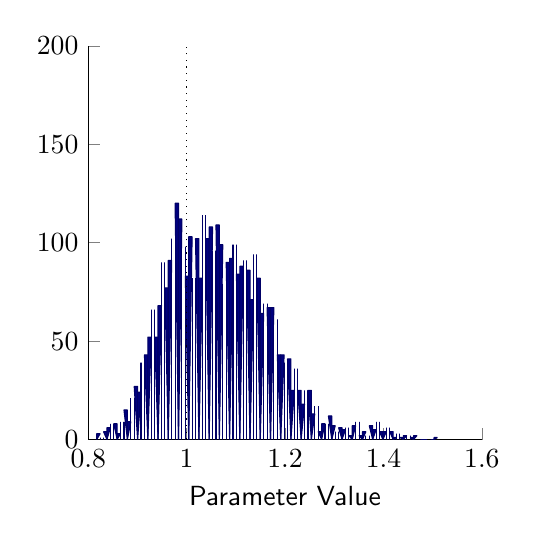
\begin{tikzpicture}

\begin{axis}[%
width=5cm,
height=5cm,
colormap/jet,
scale only axis,
xmin=0.8,
xmax=1.6,
xlabel={Parameter Value},
ymin=0,
ymax=200,
axis x line*=bottom,
axis y line*=left
]

\addplot[area legend,patch,forget plot]
table[row sep=crcr, point meta=\thisrow{c}]{
x y c\\
0.817354257272146 0 1 \\
0.817354257272146 3 1 \\
0.82427725697777 3 1 \\
0.82427725697777 0 1 \\
0.82427725697777 0 1 \\
0.82427725697777 1 1 \\
0.831200256683394 1 1 \\
0.831200256683394 0 1 \\
0.831200256683394 0 1 \\
0.831200256683394 4 1 \\
0.838123256389017 4 1 \\
0.838123256389017 0 1 \\
0.838123256389017 0 1 \\
0.838123256389017 6 1 \\
0.845046256094641 6 1 \\
0.845046256094641 0 1 \\
0.845046256094641 0 1 \\
0.845046256094641 8 1 \\
0.851969255800265 8 1 \\
0.851969255800265 0 1 \\
0.851969255800265 0 1 \\
0.851969255800265 8 1 \\
0.858892255505889 8 1 \\
0.858892255505889 0 1 \\
0.858892255505889 0 1 \\
0.858892255505889 3 1 \\
0.865815255211513 3 1 \\
0.865815255211513 0 1 \\
0.865815255211513 0 1 \\
0.865815255211513 9 1 \\
0.872738254917136 9 1 \\
0.872738254917136 0 1 \\
0.872738254917136 0 1 \\
0.872738254917136 15 1 \\
0.87966125462276 15 1 \\
0.87966125462276 0 1 \\
0.87966125462276 0 1 \\
0.87966125462276 9 1 \\
0.886584254328384 9 1 \\
0.886584254328384 0 1 \\
0.886584254328384 0 1 \\
0.886584254328384 21 1 \\
0.893507254034008 21 1 \\
0.893507254034008 0 1 \\
0.893507254034008 0 1 \\
0.893507254034008 27 1 \\
0.900430253739631 27 1 \\
0.900430253739631 0 1 \\
0.900430253739631 0 1 \\
0.900430253739631 24 1 \\
0.907353253445255 24 1 \\
0.907353253445255 0 1 \\
0.907353253445255 0 1 \\
0.907353253445255 39 1 \\
0.914276253150879 39 1 \\
0.914276253150879 0 1 \\
0.914276253150879 0 1 \\
0.914276253150879 43 1 \\
0.921199252856503 43 1 \\
0.921199252856503 0 1 \\
0.921199252856503 0 1 \\
0.921199252856503 52 1 \\
0.928122252562127 52 1 \\
0.928122252562127 0 1 \\
0.928122252562127 0 1 \\
0.928122252562127 66 1 \\
0.93504525226775 66 1 \\
0.93504525226775 0 1 \\
0.93504525226775 0 1 \\
0.93504525226775 52 1 \\
0.941968251973374 52 1 \\
0.941968251973374 0 1 \\
0.941968251973374 0 1 \\
0.941968251973374 68 1 \\
0.948891251678998 68 1 \\
0.948891251678998 0 1 \\
0.948891251678998 0 1 \\
0.948891251678998 90 1 \\
0.955814251384622 90 1 \\
0.955814251384622 0 1 \\
0.955814251384622 0 1 \\
0.955814251384622 77 1 \\
0.962737251090246 77 1 \\
0.962737251090246 0 1 \\
0.962737251090246 0 1 \\
0.962737251090246 91 1 \\
0.969660250795869 91 1 \\
0.969660250795869 0 1 \\
0.969660250795869 0 1 \\
0.969660250795869 102 1 \\
0.976583250501493 102 1 \\
0.976583250501493 0 1 \\
0.976583250501493 0 1 \\
0.976583250501493 120 1 \\
0.983506250207117 120 1 \\
0.983506250207117 0 1 \\
0.983506250207117 0 1 \\
0.983506250207117 112 1 \\
0.990429249912741 112 1 \\
0.990429249912741 0 1 \\
0.990429249912741 0 1 \\
0.990429249912741 98 1 \\
0.997352249618365 98 1 \\
0.997352249618365 0 1 \\
0.997352249618365 0 1 \\
0.997352249618365 83 1 \\
1.00427524932399 83 1 \\
1.00427524932399 0 1 \\
1.00427524932399 0 1 \\
1.00427524932399 103 1 \\
1.01119824902961 103 1 \\
1.01119824902961 0 1 \\
1.01119824902961 0 1 \\
1.01119824902961 82 1 \\
1.01812124873524 82 1 \\
1.01812124873524 0 1 \\
1.01812124873524 0 1 \\
1.01812124873524 102 1 \\
1.02504424844086 102 1 \\
1.02504424844086 0 1 \\
1.02504424844086 0 1 \\
1.02504424844086 82 1 \\
1.03196724814648 82 1 \\
1.03196724814648 0 1 \\
1.03196724814648 0 1 \\
1.03196724814648 114 1 \\
1.03889024785211 114 1 \\
1.03889024785211 0 1 \\
1.03889024785211 0 1 \\
1.03889024785211 102 1 \\
1.04581324755773 102 1 \\
1.04581324755773 0 1 \\
1.04581324755773 0 1 \\
1.04581324755773 108 1 \\
1.05273624726335 108 1 \\
1.05273624726335 0 1 \\
1.05273624726335 0 1 \\
1.05273624726335 96 1 \\
1.05965924696898 96 1 \\
1.05965924696898 0 1 \\
1.05965924696898 0 1 \\
1.05965924696898 109 1 \\
1.0665822466746 109 1 \\
1.0665822466746 0 1 \\
1.0665822466746 0 1 \\
1.0665822466746 99 1 \\
1.07350524638023 99 1 \\
1.07350524638023 0 1 \\
1.07350524638023 0 1 \\
1.07350524638023 79 1 \\
1.08042824608585 79 1 \\
1.08042824608585 0 1 \\
1.08042824608585 0 1 \\
1.08042824608585 90 1 \\
1.08735124579147 90 1 \\
1.08735124579147 0 1 \\
1.08735124579147 0 1 \\
1.08735124579147 92 1 \\
1.0942742454971 92 1 \\
1.0942742454971 0 1 \\
1.0942742454971 0 1 \\
1.0942742454971 99 1 \\
1.10119724520272 99 1 \\
1.10119724520272 0 1 \\
1.10119724520272 0 1 \\
1.10119724520272 84 1 \\
1.10812024490834 84 1 \\
1.10812024490834 0 1 \\
1.10812024490835 0 1 \\
1.10812024490835 88 1 \\
1.11504324461397 88 1 \\
1.11504324461397 0 1 \\
1.11504324461397 0 1 \\
1.11504324461397 91 1 \\
1.12196624431959 91 1 \\
1.12196624431959 0 1 \\
1.12196624431959 0 1 \\
1.12196624431959 86 1 \\
1.12888924402522 86 1 \\
1.12888924402522 0 1 \\
1.12888924402522 0 1 \\
1.12888924402522 71 1 \\
1.13581224373084 71 1 \\
1.13581224373084 0 1 \\
1.13581224373084 0 1 \\
1.13581224373084 94 1 \\
1.14273524343646 94 1 \\
1.14273524343646 0 1 \\
1.14273524343646 0 1 \\
1.14273524343646 82 1 \\
1.14965824314209 82 1 \\
1.14965824314209 0 1 \\
1.14965824314209 0 1 \\
1.14965824314209 64 1 \\
1.15658124284771 64 1 \\
1.15658124284771 0 1 \\
1.15658124284771 0 1 \\
1.15658124284771 69 1 \\
1.16350424255334 69 1 \\
1.16350424255334 0 1 \\
1.16350424255334 0 1 \\
1.16350424255334 67 1 \\
1.17042724225896 67 1 \\
1.17042724225896 0 1 \\
1.17042724225896 0 1 \\
1.17042724225896 67 1 \\
1.17735024196458 67 1 \\
1.17735024196458 0 1 \\
1.17735024196458 0 1 \\
1.17735024196458 61 1 \\
1.18427324167021 61 1 \\
1.18427324167021 0 1 \\
1.18427324167021 0 1 \\
1.18427324167021 43 1 \\
1.19119624137583 43 1 \\
1.19119624137583 0 1 \\
1.19119624137583 0 1 \\
1.19119624137583 43 1 \\
1.19811924108145 43 1 \\
1.19811924108145 0 1 \\
1.19811924108145 0 1 \\
1.19811924108145 39 1 \\
1.20504224078708 39 1 \\
1.20504224078708 0 1 \\
1.20504224078708 0 1 \\
1.20504224078708 41 1 \\
1.2119652404927 41 1 \\
1.2119652404927 0 1 \\
1.2119652404927 0 1 \\
1.2119652404927 25 1 \\
1.21888824019833 25 1 \\
1.21888824019833 0 1 \\
1.21888824019833 0 1 \\
1.21888824019833 36 1 \\
1.22581123990395 36 1 \\
1.22581123990395 0 1 \\
1.22581123990395 0 1 \\
1.22581123990395 25 1 \\
1.23273423960957 25 1 \\
1.23273423960957 0 1 \\
1.23273423960957 0 1 \\
1.23273423960957 18 1 \\
1.2396572393152 18 1 \\
1.2396572393152 0 1 \\
1.2396572393152 0 1 \\
1.2396572393152 25 1 \\
1.24658023902082 25 1 \\
1.24658023902082 0 1 \\
1.24658023902082 0 1 \\
1.24658023902082 25 1 \\
1.25350323872644 25 1 \\
1.25350323872644 0 1 \\
1.25350323872644 0 1 \\
1.25350323872644 13 1 \\
1.26042623843207 13 1 \\
1.26042623843207 0 1 \\
1.26042623843207 0 1 \\
1.26042623843207 17 1 \\
1.26734923813769 17 1 \\
1.26734923813769 0 1 \\
1.26734923813769 0 1 \\
1.26734923813769 4 1 \\
1.27427223784332 4 1 \\
1.27427223784332 0 1 \\
1.27427223784332 0 1 \\
1.27427223784332 8 1 \\
1.28119523754894 8 1 \\
1.28119523754894 0 1 \\
1.28119523754894 0 1 \\
1.28119523754894 8 1 \\
1.28811823725456 8 1 \\
1.28811823725456 0 1 \\
1.28811823725456 0 1 \\
1.28811823725456 12 1 \\
1.29504123696019 12 1 \\
1.29504123696019 0 1 \\
1.29504123696019 0 1 \\
1.29504123696019 7 1 \\
1.30196423666581 7 1 \\
1.30196423666581 0 1 \\
1.30196423666581 0 1 \\
1.30196423666581 4 1 \\
1.30888723637143 4 1 \\
1.30888723637143 0 1 \\
1.30888723637143 0 1 \\
1.30888723637143 6 1 \\
1.31581023607706 6 1 \\
1.31581023607706 0 1 \\
1.31581023607706 0 1 \\
1.31581023607706 5 1 \\
1.32273323578268 5 1 \\
1.32273323578268 0 1 \\
1.32273323578268 0 1 \\
1.32273323578268 6 1 \\
1.32965623548831 6 1 \\
1.32965623548831 0 1 \\
1.32965623548831 0 1 \\
1.32965623548831 2 1 \\
1.33657923519393 2 1 \\
1.33657923519393 0 1 \\
1.33657923519393 0 1 \\
1.33657923519393 7 1 \\
1.34350223489955 7 1 \\
1.34350223489955 0 1 \\
1.34350223489955 0 1 \\
1.34350223489955 9 1 \\
1.35042523460518 9 1 \\
1.35042523460518 0 1 \\
1.35042523460518 0 1 \\
1.35042523460518 2 1 \\
1.3573482343108 2 1 \\
1.3573482343108 0 1 \\
1.3573482343108 0 1 \\
1.3573482343108 4 1 \\
1.36427123401643 4 1 \\
1.36427123401643 0 1 \\
1.36427123401643 0 1 \\
1.36427123401643 2 1 \\
1.37119423372205 2 1 \\
1.37119423372205 0 1 \\
1.37119423372205 0 1 \\
1.37119423372205 7 1 \\
1.37811723342767 7 1 \\
1.37811723342767 0 1 \\
1.37811723342767 0 1 \\
1.37811723342767 5 1 \\
1.3850402331333 5 1 \\
1.3850402331333 0 1 \\
1.3850402331333 0 1 \\
1.3850402331333 9 1 \\
1.39196323283892 9 1 \\
1.39196323283892 0 1 \\
1.39196323283892 0 1 \\
1.39196323283892 4 1 \\
1.39888623254454 4 1 \\
1.39888623254454 0 1 \\
1.39888623254454 0 1 \\
1.39888623254454 4 1 \\
1.40580923225017 4 1 \\
1.40580923225017 0 1 \\
1.40580923225017 0 1 \\
1.40580923225017 6 1 \\
1.41273223195579 6 1 \\
1.41273223195579 0 1 \\
1.41273223195579 0 1 \\
1.41273223195579 4 1 \\
1.41965523166142 4 1 \\
1.41965523166142 0 1 \\
1.41965523166142 0 1 \\
1.41965523166142 1 1 \\
1.42657823136704 1 1 \\
1.42657823136704 0 1 \\
1.42657823136704 0 1 \\
1.42657823136704 3 1 \\
1.43350123107266 3 1 \\
1.43350123107266 0 1 \\
1.43350123107266 0 1 \\
1.43350123107266 1 1 \\
1.44042423077829 1 1 \\
1.44042423077829 0 1 \\
1.44042423077829 0 1 \\
1.44042423077829 2 1 \\
1.44734723048391 2 1 \\
1.44734723048391 0 1 \\
1.44734723048391 0 1 \\
1.44734723048391 2 1 \\
1.45427023018953 2 1 \\
1.45427023018953 0 1 \\
1.45427023018953 0 1 \\
1.45427023018953 1 1 \\
1.46119322989516 1 1 \\
1.46119322989516 0 1 \\
1.46119322989516 0 1 \\
1.46119322989516 2 1 \\
1.46811622960078 2 1 \\
1.46811622960078 0 1 \\
1.46811622960078 0 1 \\
1.46811622960078 0 1 \\
1.47503922930641 0 1 \\
1.47503922930641 0 1 \\
1.47503922930641 0 1 \\
1.47503922930641 0 1 \\
1.48196222901203 0 1 \\
1.48196222901203 0 1 \\
1.48196222901203 0 1 \\
1.48196222901203 0 1 \\
1.48888522871765 0 1 \\
1.48888522871765 0 1 \\
1.48888522871765 0 1 \\
1.48888522871765 0 1 \\
1.49580822842328 0 1 \\
1.49580822842328 0 1 \\
1.49580822842328 0 1 \\
1.49580822842328 0 1 \\
1.5027312281289 0 1 \\
1.5027312281289 0 1 \\
1.5027312281289 0 1 \\
1.5027312281289 1 1 \\
1.50965422783452 1 1 \\
1.50965422783452 0 1 \\
};

\addplot [
color=black,
dotted,
forget plot
]
table[row sep=crcr]{
1 0\\
1 200\\
};
\end{axis}
\end{tikzpicture}% } \\
\subfloat[PG-RBS (N=100)]{ % This file was created by matlab2tikz v0.4.4 running on MATLAB 7.13.
% Copyright (c) 2008--2013, Nico Schlömer <nico.schloemer@gmail.com>
% All rights reserved.
% 
% The latest updates can be retrieved from
%   http://www.mathworks.com/matlabcentral/fileexchange/22022-matlab2tikz
% where you can also make suggestions and rate matlab2tikz.
% 
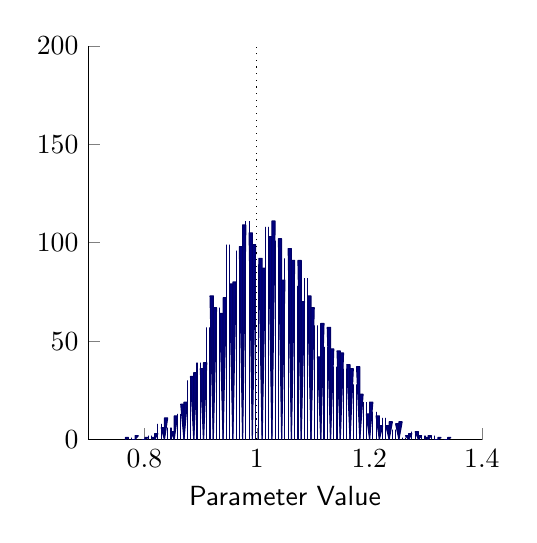
\begin{tikzpicture}

\begin{axis}[%
width=5cm,
height=5cm,
colormap/jet,
scale only axis,
xmin=0.7,
xmax=1.4,
xlabel={Parameter Value},
ymin=0,
ymax=200,
axis x line*=bottom,
axis y line*=left
]

\addplot[area legend,patch,forget plot]
table[row sep=crcr, point meta=\thisrow{c}]{
x y c\\
0.766108479366861 0 1 \\
0.766108479366861 1 1 \\
0.771898170514086 1 1 \\
0.771898170514086 0 1 \\
0.771898170514086 0 1 \\
0.771898170514086 1 1 \\
0.777687861661311 1 1 \\
0.777687861661311 0 1 \\
0.777687861661311 0 1 \\
0.777687861661311 0 1 \\
0.783477552808536 0 1 \\
0.783477552808536 0 1 \\
0.783477552808536 0 1 \\
0.783477552808536 2 1 \\
0.789267243955761 2 1 \\
0.789267243955761 0 1 \\
0.789267243955761 0 1 \\
0.789267243955761 0 1 \\
0.795056935102985 0 1 \\
0.795056935102985 0 1 \\
0.795056935102985 0 1 \\
0.795056935102985 0 1 \\
0.80084662625021 0 1 \\
0.80084662625021 0 1 \\
0.80084662625021 0 1 \\
0.80084662625021 1 1 \\
0.806636317397435 1 1 \\
0.806636317397435 0 1 \\
0.806636317397435 0 1 \\
0.806636317397435 2 1 \\
0.81242600854466 2 1 \\
0.81242600854466 0 1 \\
0.81242600854466 0 1 \\
0.81242600854466 1 1 \\
0.818215699691885 1 1 \\
0.818215699691885 0 1 \\
0.818215699691885 0 1 \\
0.818215699691885 3 1 \\
0.824005390839109 3 1 \\
0.824005390839109 0 1 \\
0.824005390839109 0 1 \\
0.824005390839109 8 1 \\
0.829795081986334 8 1 \\
0.829795081986334 0 1 \\
0.829795081986334 0 1 \\
0.829795081986334 6 1 \\
0.835584773133559 6 1 \\
0.835584773133559 0 1 \\
0.835584773133559 0 1 \\
0.835584773133559 11 1 \\
0.841374464280784 11 1 \\
0.841374464280784 0 1 \\
0.841374464280784 0 1 \\
0.841374464280784 6 1 \\
0.847164155428009 6 1 \\
0.847164155428009 0 1 \\
0.847164155428009 0 1 \\
0.847164155428009 4 1 \\
0.852953846575233 4 1 \\
0.852953846575233 0 1 \\
0.852953846575233 0 1 \\
0.852953846575233 12 1 \\
0.858743537722458 12 1 \\
0.858743537722458 0 1 \\
0.858743537722458 0 1 \\
0.858743537722458 13 1 \\
0.864533228869683 13 1 \\
0.864533228869683 0 1 \\
0.864533228869683 0 1 \\
0.864533228869683 18 1 \\
0.870322920016908 18 1 \\
0.870322920016908 0 1 \\
0.870322920016908 0 1 \\
0.870322920016908 19 1 \\
0.876112611164133 19 1 \\
0.876112611164133 0 1 \\
0.876112611164133 0 1 \\
0.876112611164133 30 1 \\
0.881902302311357 30 1 \\
0.881902302311357 0 1 \\
0.881902302311357 0 1 \\
0.881902302311357 32 1 \\
0.887691993458582 32 1 \\
0.887691993458582 0 1 \\
0.887691993458582 0 1 \\
0.887691993458582 34 1 \\
0.893481684605807 34 1 \\
0.893481684605807 0 1 \\
0.893481684605807 0 1 \\
0.893481684605807 39 1 \\
0.899271375753032 39 1 \\
0.899271375753032 0 1 \\
0.899271375753032 0 1 \\
0.899271375753032 36 1 \\
0.905061066900257 36 1 \\
0.905061066900257 0 1 \\
0.905061066900257 0 1 \\
0.905061066900257 39 1 \\
0.910850758047481 39 1 \\
0.910850758047481 0 1 \\
0.910850758047481 0 1 \\
0.910850758047481 57 1 \\
0.916640449194706 57 1 \\
0.916640449194706 0 1 \\
0.916640449194706 0 1 \\
0.916640449194706 73 1 \\
0.922430140341931 73 1 \\
0.922430140341931 0 1 \\
0.922430140341931 0 1 \\
0.922430140341931 67 1 \\
0.928219831489156 67 1 \\
0.928219831489156 0 1 \\
0.928219831489156 0 1 \\
0.928219831489156 67 1 \\
0.934009522636381 67 1 \\
0.934009522636381 0 1 \\
0.93400952263638 0 1 \\
0.93400952263638 64 1 \\
0.939799213783605 64 1 \\
0.939799213783605 0 1 \\
0.939799213783605 0 1 \\
0.939799213783605 72 1 \\
0.94558890493083 72 1 \\
0.94558890493083 0 1 \\
0.94558890493083 0 1 \\
0.94558890493083 99 1 \\
0.951378596078055 99 1 \\
0.951378596078055 0 1 \\
0.951378596078055 0 1 \\
0.951378596078055 79 1 \\
0.95716828722528 79 1 \\
0.95716828722528 0 1 \\
0.95716828722528 0 1 \\
0.95716828722528 80 1 \\
0.962957978372505 80 1 \\
0.962957978372505 0 1 \\
0.962957978372505 0 1 \\
0.962957978372505 96 1 \\
0.968747669519729 96 1 \\
0.968747669519729 0 1 \\
0.968747669519729 0 1 \\
0.968747669519729 98 1 \\
0.974537360666954 98 1 \\
0.974537360666954 0 1 \\
0.974537360666954 0 1 \\
0.974537360666954 109 1 \\
0.980327051814179 109 1 \\
0.980327051814179 0 1 \\
0.980327051814179 0 1 \\
0.980327051814179 111 1 \\
0.986116742961404 111 1 \\
0.986116742961404 0 1 \\
0.986116742961404 0 1 \\
0.986116742961404 105 1 \\
0.991906434108629 105 1 \\
0.991906434108629 0 1 \\
0.991906434108629 0 1 \\
0.991906434108629 99 1 \\
0.997696125255853 99 1 \\
0.997696125255853 0 1 \\
0.997696125255853 0 1 \\
0.997696125255853 89 1 \\
1.00348581640308 89 1 \\
1.00348581640308 0 1 \\
1.00348581640308 0 1 \\
1.00348581640308 92 1 \\
1.0092755075503 92 1 \\
1.0092755075503 0 1 \\
1.0092755075503 0 1 \\
1.0092755075503 87 1 \\
1.01506519869753 87 1 \\
1.01506519869753 0 1 \\
1.01506519869753 0 1 \\
1.01506519869753 108 1 \\
1.02085488984475 108 1 \\
1.02085488984475 0 1 \\
1.02085488984475 0 1 \\
1.02085488984475 103 1 \\
1.02664458099198 103 1 \\
1.02664458099198 0 1 \\
1.02664458099198 0 1 \\
1.02664458099198 111 1 \\
1.0324342721392 111 1 \\
1.0324342721392 0 1 \\
1.0324342721392 0 1 \\
1.0324342721392 101 1 \\
1.03822396328643 101 1 \\
1.03822396328643 0 1 \\
1.03822396328643 0 1 \\
1.03822396328643 102 1 \\
1.04401365443365 102 1 \\
1.04401365443365 0 1 \\
1.04401365443365 0 1 \\
1.04401365443365 81 1 \\
1.04980334558088 81 1 \\
1.04980334558088 0 1 \\
1.04980334558088 0 1 \\
1.04980334558088 92 1 \\
1.0555930367281 92 1 \\
1.0555930367281 0 1 \\
1.0555930367281 0 1 \\
1.0555930367281 97 1 \\
1.06138272787533 97 1 \\
1.06138272787533 0 1 \\
1.06138272787533 0 1 \\
1.06138272787533 91 1 \\
1.06717241902255 91 1 \\
1.06717241902255 0 1 \\
1.06717241902255 0 1 \\
1.06717241902255 78 1 \\
1.07296211016978 78 1 \\
1.07296211016978 0 1 \\
1.07296211016978 0 1 \\
1.07296211016978 91 1 \\
1.078751801317 91 1 \\
1.078751801317 0 1 \\
1.078751801317 0 1 \\
1.078751801317 70 1 \\
1.08454149246423 70 1 \\
1.08454149246423 0 1 \\
1.08454149246423 0 1 \\
1.08454149246423 82 1 \\
1.09033118361145 82 1 \\
1.09033118361145 0 1 \\
1.09033118361145 0 1 \\
1.09033118361145 73 1 \\
1.09612087475867 73 1 \\
1.09612087475867 0 1 \\
1.09612087475867 0 1 \\
1.09612087475867 67 1 \\
1.1019105659059 67 1 \\
1.1019105659059 0 1 \\
1.1019105659059 0 1 \\
1.1019105659059 58 1 \\
1.10770025705312 58 1 \\
1.10770025705312 0 1 \\
1.10770025705312 0 1 \\
1.10770025705312 42 1 \\
1.11348994820035 42 1 \\
1.11348994820035 0 1 \\
1.11348994820035 0 1 \\
1.11348994820035 59 1 \\
1.11927963934757 59 1 \\
1.11927963934757 0 1 \\
1.11927963934757 0 1 \\
1.11927963934757 47 1 \\
1.1250693304948 47 1 \\
1.1250693304948 0 1 \\
1.1250693304948 0 1 \\
1.1250693304948 57 1 \\
1.13085902164202 57 1 \\
1.13085902164202 0 1 \\
1.13085902164202 0 1 \\
1.13085902164202 46 1 \\
1.13664871278925 46 1 \\
1.13664871278925 0 1 \\
1.13664871278925 0 1 \\
1.13664871278925 37 1 \\
1.14243840393647 37 1 \\
1.14243840393647 0 1 \\
1.14243840393647 0 1 \\
1.14243840393647 45 1 \\
1.1482280950837 45 1 \\
1.1482280950837 0 1 \\
1.1482280950837 0 1 \\
1.1482280950837 44 1 \\
1.15401778623092 44 1 \\
1.15401778623092 0 1 \\
1.15401778623092 0 1 \\
1.15401778623092 36 1 \\
1.15980747737815 36 1 \\
1.15980747737815 0 1 \\
1.15980747737815 0 1 \\
1.15980747737815 38 1 \\
1.16559716852537 38 1 \\
1.16559716852537 0 1 \\
1.16559716852537 0 1 \\
1.16559716852537 36 1 \\
1.1713868596726 36 1 \\
1.1713868596726 0 1 \\
1.1713868596726 0 1 \\
1.1713868596726 28 1 \\
1.17717655081982 28 1 \\
1.17717655081982 0 1 \\
1.17717655081982 0 1 \\
1.17717655081982 37 1 \\
1.18296624196705 37 1 \\
1.18296624196705 0 1 \\
1.18296624196705 0 1 \\
1.18296624196705 23 1 \\
1.18875593311427 23 1 \\
1.18875593311427 0 1 \\
1.18875593311427 0 1 \\
1.18875593311427 19 1 \\
1.1945456242615 19 1 \\
1.1945456242615 0 1 \\
1.1945456242615 0 1 \\
1.1945456242615 13 1 \\
1.20033531540872 13 1 \\
1.20033531540872 0 1 \\
1.20033531540872 0 1 \\
1.20033531540872 19 1 \\
1.20612500655595 19 1 \\
1.20612500655595 0 1 \\
1.20612500655595 0 1 \\
1.20612500655595 14 1 \\
1.21191469770317 14 1 \\
1.21191469770317 0 1 \\
1.21191469770317 0 1 \\
1.21191469770317 12 1 \\
1.2177043888504 12 1 \\
1.2177043888504 0 1 \\
1.2177043888504 0 1 \\
1.2177043888504 7 1 \\
1.22349407999762 7 1 \\
1.22349407999762 0 1 \\
1.22349407999762 0 1 \\
1.22349407999762 11 1 \\
1.22928377114485 11 1 \\
1.22928377114485 0 1 \\
1.22928377114485 0 1 \\
1.22928377114485 7 1 \\
1.23507346229207 7 1 \\
1.23507346229207 0 1 \\
1.23507346229207 0 1 \\
1.23507346229207 9 1 \\
1.24086315343929 9 1 \\
1.24086315343929 0 1 \\
1.24086315343929 0 1 \\
1.24086315343929 5 1 \\
1.24665284458652 5 1 \\
1.24665284458652 0 1 \\
1.24665284458652 0 1 \\
1.24665284458652 8 1 \\
1.25244253573374 8 1 \\
1.25244253573374 0 1 \\
1.25244253573374 0 1 \\
1.25244253573374 9 1 \\
1.25823222688097 9 1 \\
1.25823222688097 0 1 \\
1.25823222688097 0 1 \\
1.25823222688097 1 1 \\
1.26402191802819 1 1 \\
1.26402191802819 0 1 \\
1.26402191802819 0 1 \\
1.26402191802819 2 1 \\
1.26981160917542 2 1 \\
1.26981160917542 0 1 \\
1.26981160917542 0 1 \\
1.26981160917542 3 1 \\
1.27560130032264 3 1 \\
1.27560130032264 0 1 \\
1.27560130032264 0 1 \\
1.27560130032264 4 1 \\
1.28139099146987 4 1 \\
1.28139099146987 0 1 \\
1.28139099146987 0 1 \\
1.28139099146987 4 1 \\
1.28718068261709 4 1 \\
1.28718068261709 0 1 \\
1.28718068261709 0 1 \\
1.28718068261709 2 1 \\
1.29297037376432 2 1 \\
1.29297037376432 0 1 \\
1.29297037376432 0 1 \\
1.29297037376432 2 1 \\
1.29876006491154 2 1 \\
1.29876006491154 0 1 \\
1.29876006491154 0 1 \\
1.29876006491154 1 1 \\
1.30454975605877 1 1 \\
1.30454975605877 0 1 \\
1.30454975605877 0 1 \\
1.30454975605877 2 1 \\
1.31033944720599 2 1 \\
1.31033944720599 0 1 \\
1.31033944720599 0 1 \\
1.31033944720599 2 1 \\
1.31612913835322 2 1 \\
1.31612913835322 0 1 \\
1.31612913835322 0 1 \\
1.31612913835322 0 1 \\
1.32191882950044 0 1 \\
1.32191882950044 0 1 \\
1.32191882950044 0 1 \\
1.32191882950044 1 1 \\
1.32770852064767 1 1 \\
1.32770852064767 0 1 \\
1.32770852064767 0 1 \\
1.32770852064767 0 1 \\
1.33349821179489 0 1 \\
1.33349821179489 0 1 \\
1.33349821179489 0 1 \\
1.33349821179489 0 1 \\
1.33928790294212 0 1 \\
1.33928790294212 0 1 \\
1.33928790294212 0 1 \\
1.33928790294212 1 1 \\
1.34507759408934 1 1 \\
1.34507759408934 0 1 \\
};

\addplot [
color=black,
dotted,
forget plot
]
table[row sep=crcr]{
1 0\\
1 200\\
};
\end{axis}
\end{tikzpicture}% }
\caption{Posterior sample histograms.}
\label{fig:sample_hist}
\end{figure}


\section{Conclusions}




\appendix

\section{Manipulations of the Particle Gibbs Extended Target Distribution}

\subsection{Extended Target Distribution}

The particle MCMC extended target distribution is,
%
\begin{IEEEeqnarray}{rCl}
 \ed(\pr, \lsset{1:\timax}, \anset{2:\timax}, \aifinal) & = & \frac{1}{\nump^\timax} \den(\pr, \ls{1:\timax}\pss{\ai{1:\timax}}|\ob{1:\timax}) \nonumber \\
  & & \qquad  \times \prod_{i\ne\ai{1}} \pd(\ls{1}\pss{i}) \prod_{\ti=1}^{\timax} \left[ \prod_{i\ne\ai{\ti}} \frac{ \pw{\ti-1}\pss{\an{\ti}\pss{i}} }{ \sum_j \pw{\ti-1}\pss{j} } \pd(\ls{\ti}\pss{i}|\ls{\ti-1}\pss{\an{\ti}\pss{i}}) \right] \label{eq:extended_dist_v1}     .
\end{IEEEeqnarray}
%
The necessary rearrangement of this distribution is achieved by expanding the posterior term using Bayes rule,
%
\begin{IEEEeqnarray}{rCl}
 \den(\pr, \ls{1:\timax}\pss{\ai{1:\timax}}|\ob{1:\timax}) & = & \frac{ \den(\ob{1:\timax} | \ls{1:\timax}\pss{\ai{1:\timax}}, \pr) \den(\ls{1:\timax}\pss{\ai{1:\timax}}|\pr) \den(\pr|\ob{1:\timax}) }{ \den(\ob{1:\timax}|\pr) } \nonumber \\
 & = & \frac{\den(\pr|\ob{1:\timax})}{\den(\ob{1:\timax}|\pr)} \td(\ls{1}\pss{\ai{1}}) \od(\ob{1}|\ls{1}\pss{\ai{1}}) \prod \td(\ls{\ti}\pss{\ai{\ti}}|\ls{\ti-1}\pss{\an{\ti}\pss{\ai{\ti}}}) \od(\ob{\ti}|\ls{\ti}\pss{\ai{\ti}}) \nonumber       ,
\end{IEEEeqnarray}
%
and then repeatedly applying the following identity,
%
\begin{IEEEeqnarray}{rCl}
 \td(\ls{\ti}\pss{i}|\ls{\ti-1}\pss{\an{\ti}\pss{i}}) \od(\ob{\ti}|\ls{\ti}\pss{i}) & = & \pw{\ti}\pss{i} \pd(\ls{\ti}\pss{i}|\ls{\ti-1}\pss{\an{\ti}\pss{i}}) \nonumber \\
 \td(\ls{1}\pss{i}) \od(\ob{1}|\ls{1}\pss{i}) & = & \pw{1}\pss{i} \pd(\ls{1}\pss{i}) \label{eq:pmcmc_id}   .
\end{IEEEeqnarray}
%
This leads us to,
%
\begin{IEEEeqnarray}{rCl}
 \ed(\pr, \lsset{1:\timax}, \anset{2:\timax}, \aifinal) & = & \frac{\den(\pr|\ob{1:\timax})}{\nump^\timax} \frac{\sum_j \pw{\timax}\pss{j}}{\den(\ob{1:\timax}|\pr)} \nonumber \\
 & & \times \prod_{i} \pd(\ls{1}\pss{i}) \prod_{\ti=1}^{\timax} \left[ \prod_{i} \frac{ \pw{\ti-1}\pss{\an{\ti}\pss{i}} }{ \sum_j \pw{\ti-1}\pss{j} } \pd(\ls{\ti}\pss{i}|\ls{\ti-1}\pss{\an{\ti}\pss{i}}) \right] \nonumber \\
 & & \times \frac{ \pw{\timax}\pss{\aifinal} }{ \sum_j \pw{\timax}\pss{j} } \label{eq:extended_dist_v2}     .
\end{IEEEeqnarray}
%
This is the form we need for particle marginal Metropolis-Hastings.



\subsection{Particle Gibbs with Backward Simulation}

In a basic particle Gibbs sampler, we alternately sample $\aifinal$ and $\lsset{1:\timax}\pss{\notai{1:\timax}}, \anset{2:\timax}\pss{\notai{1:\timax}}$. When doing ordinary backward simulation, we add an additional set of steps. Passing backwards through time from $\ti=\timax$ to $\ti=1$, we sample from,
%
\begin{IEEEeqnarray}{rCl}
 \ed(\an{\ti}\pss{\ai{\ti}} | \pr, \lsset{1:\ti-1}, \anset{1:\ti-1}, \ls{\ti:\timax}\pss{\ai{\ti:\timax}}, \an{\ti+1:\timax}\pss{\ai{\ti+1:\timax}}, \aifinal)      .
\end{IEEEeqnarray}
%
This is a collapsed Gibbs move. We need to manipulate the extended target distribution as follows. Starting with \eqref{eq:extended_dist_v1}, first marginalise the future variables by alternately integrating out the final state and then summing over the final ancestor indexes. Then expand the posterior term using Bayes rule and use \eqref{eq:pmcmc_id} repeatedly again,
%
\begin{IEEEeqnarray}{rCl}
 \IEEEeqnarraymulticol{3}{l}{ \ed(\pr, \lsset{1:\ti-1}, \anset{2:\ti-1}, \ls{\ti:\timax}\pss{\ai{\ti:\timax}}, \an{\ti:\timax}\pss{\ai{\ti:\timax}}, \aifinal) } \nonumber \\
 \qquad \qquad & = & \frac{\den(\pr|\ob{1:\timax})}{\nump^{\timax}} \den(\ls{1:\timax}\pss{\ai{1:\timax}}|\ob{1:\timax},\pr) \nonumber \\
  & & \times \prod_{i\ne\ai{1}} \pd(\ls{1}\pss{i}) \prod_{k=1}^{\ti-1} \left[ \prod_{i\ne\ai{k}} \frac{ \pw{k-1}\pss{\an{k}\pss{i}} }{ \sum_j \pw{k-1}\pss{j} } \pd(\ls{k}\pss{i}|\ls{k-1}\pss{\an{k}\pss{i}}) \right] \nonumber \\
 & = & \frac{\den(\pr|\ob{1:\timax})}{\nump^{\timax}} \frac{ \den(\ob{\ti:\timax}|\ls{\ti:\timax}\pss{\ai{\ti:\timax}},\pr) }{ \den(\ob{1:\timax}|\pr) } \nonumber \\
 & & \times \prod_{i} \pd(\ls{1}\pss{i}) \prod_{k=1}^{\ti-1} \left[ \prod_{i} \frac{ \pw{k-1}\pss{\an{k}\pss{i}} }{ \sum_j \pw{k-1}\pss{j} } \pd(\ls{k}\pss{i}|\ls{k-1}\pss{\an{k}\pss{i}}) \right] \nonumber \\
 & & \times \pw{\ti}\pss{\an{\ti}\pss{\ai{\ti}}} \times \td(\ls{\ti}\pss{\ai{\ti}}|\ls{\ti-1}\pss{\an{\ti}\pss{\ai{\ti}}}) \nonumber      .
\end{IEEEeqnarray}
%
Then marginalise $\an{\ti}\pss{\ai{\ti}}$,
%
\begin{IEEEeqnarray}{rCl}
 \IEEEeqnarraymulticol{3}{l}{ \ed(\pr, \lsset{1:\ti-1}, \anset{2:\ti-1}, \ls{\ti:\timax}\pss{\ai{\ti:\timax}}, \an{\ti+1:\timax}\pss{\ai{\ti+1:\timax}}, \aifinal) } \nonumber \\
 \qquad \qquad & = & \frac{\den(\pr|\ob{1:\timax})}{\nump^{\timax}} \frac{ \den(\ob{\ti:\timax}|\ls{\ti:\timax}\pss{\ai{\ti:\timax}},\pr) }{ \den(\ob{1:\timax}|\pr) } \nonumber \\
 & & \times \prod_{i} \pd(\ls{1}\pss{i}) \prod_{k=1}^{\ti-1} \left[ \prod_{i} \frac{ \pw{k-1}\pss{\an{k}\pss{i}} }{ \sum_j \pw{k-1}\pss{j} } \pd(\ls{k}\pss{i}|\ls{k-1}\pss{\an{k}\pss{i}}) \right] \nonumber \\
 & & \times \sum_j \pw{\ti}\pss{j} \times \td(\ls{\ti}\pss{\ai{\ti}}|\ls{\ti-1}\pss{j}) \nonumber      ,
\end{IEEEeqnarray}
%
and obtain the conditional,
%
\begin{IEEEeqnarray}{rCl}
 \ed(\an{\ti}\pss{\ai{\ti}} | \pr, \lsset{1:\ti-1}, \anset{2:\ti-1}, \ls{\ti:\timax}\pss{\ai{\ti:\timax}}, \an{\ti+1:\timax}\pss{\ai{\ti+1:\timax}}, \aifinal) & = & \frac{ \pw{\ti}\pss{\an{\ti}\pss{\ai{\ti}}} \td(\ls{\ti}\pss{\ai{\ti}}|\ls{\ti-1}\pss{\an{\ti}\pss{\ai{\ti}}}) }{ \sum_j \pw{\ti}\pss{j} \td(\ls{\ti}\pss{\ai{\ti}}|\ls{\ti-1}\pss{j}) }     .
\end{IEEEeqnarray}



\subsection{Particle Gibbs with Refreshed Backward Simulation}

The change we're going to make is to replace the collapsed Gibbs steps constituting backward simulation with a new set, sampling recursively from,
%
\begin{IEEEeqnarray}{rCl}
 \ed(\ls{\ti}\pss{\ai{\ti}}, \an{\ti}\pss{\ai{\ti}} | \pr, \lsset{1:\ti-1}, \anset{1:\ti-1}, \ls{\ti+1:\timax}\pss{\ai{\ti+1:\timax}}, \an{\ti+1:\timax}\pss{\ai{\ti+1:\timax}}, \aifinal)      .
\end{IEEEeqnarray}
%
The manipulations of the extended target distribution are similar to before,
%
\begin{IEEEeqnarray}{rCl}
 \IEEEeqnarraymulticol{3}{l}{ \ed(\pr, \lsset{1:\ti-1}, \anset{1:\ti-1}, \ls{\ti:\timax}\pss{\ai{\ti:\timax}}, \an{\ti:\timax}\pss{\ai{\ti:\timax}}, \aifinal) } \nonumber \\
 \qquad \qquad & = & \frac{\den(\pr|\ob{1:\timax})}{\nump^{\timax}} \den(\ls{1:\timax}\pss{\ai{1:\timax}}|\ob{1:\timax},\pr) \nonumber \\
  & & \times \prod_{i\ne\ai{1}} \pd(\ls{1}\pss{i}) \prod_{k=1}^{\ti-1} \left[ \prod_{i\ne\ai{k}} \frac{ \pw{k-1}\pss{\an{k}\pss{i}} }{ \sum_j \pw{k-1}\pss{j} } \pd(\ls{k}\pss{i}|\ls{k-1}\pss{\an{k}\pss{i}}) \right] \nonumber \\
 & = & \frac{\den(\pr|\ob{1:\timax})}{\nump^{\timax}} \frac{ \den(\ob{\ti+1:\timax}|\ls{\ti+1:\timax}\pss{\ai{\ti+1:\timax}},\pr) }{ \den(\ob{1:\timax}|\pr) } \nonumber \\
 & & \times \prod_{i} \pd(\ls{1}\pss{i}) \prod_{k=1}^{\ti-1} \left[ \prod_{i} \frac{ \pw{k-1}\pss{\an{k}\pss{i}} }{ \sum_j \pw{k-1}\pss{j} } \pd(\ls{k}\pss{i}|\ls{k-1}\pss{\an{k}\pss{i}}) \right] \nonumber \\
 & & \times \pw{\ti}\pss{\an{\ti}\pss{\ai{\ti}}} \times \td(\ls{\ti}\pss{\ai{\ti}}|\ls{\ti-1}\pss{\an{\ti}\pss{\ai{\ti}}}) \od(\ob{\ti}|\ls{\ti}\pss{\ai{\ti}}) \td(\ls{\ti+1}\pss{\ai{\ti+1}}|\ls{\ti}\pss{\an{\ti+1}\pss{\ai{\ti+1}}}) \nonumber      .
\end{IEEEeqnarray}
%
Now marginalise both $\ls{\ti}\pss{\ai{\ti}}$ and $\an{\ti}\pss{\ai{\ti}}$,
%
\begin{IEEEeqnarray}{rCl}
 \IEEEeqnarraymulticol{3}{l}{ \ed(\pr, \lsset{1:\ti-1}, \anset{1:\ti-1}, \ls{\ti+1:\timax}\pss{\ai{\ti+1:\timax}}, \an{\ti+1:\timax}\pss{\ai{\ti+1:\timax}}, \aifinal) } \nonumber \\
 \qquad \qquad & = & \frac{\den(\pr|\ob{1:\timax})}{\nump^{\timax}} \frac{ \den(\ob{\ti+1:\timax}|\ls{\ti+1:\timax}\pss{\ai{\ti+1:\timax}},\pr) }{ \den(\ob{1:\timax}|\pr) } \nonumber \\
 & & \times \prod_{i} \pd(\ls{1}\pss{i}) \prod_{k=1}^{\ti-1} \left[ \prod_{i} \frac{ \pw{k-1}\pss{\an{k}\pss{i}} }{ \sum_j \pw{k-1}\pss{j} } \pd(\ls{k}\pss{i}|\ls{k-1}\pss{\an{k}\pss{i}}) \right] \nonumber \\
 & & \times \sum_j \pw{\ti}\pss{j} \int \td(\ls{\ti}\pss{\ai{\ti}}|\ls{\ti-1}\pss{j}) \od(\ob{\ti}|\ls{\ti}\pss{\ai{\ti}}) \td(\ls{\ti+1}\pss{\ai{\ti+1}}|\ls{\ti}\pss{\ai{\ti}}) d\ls{\ti}\pss{\ai{\ti}} \nonumber      ,
\end{IEEEeqnarray}
%
and obtain the conditional,
%
\begin{IEEEeqnarray}{rCl}
 \IEEEeqnarraymulticol{3}{l}{ \ed(\ls{\ti}\pss{\ai{\ti}}, \an{\ti}\pss{\ai{\ti}} | \pr, \lsset{1:\ti-1}, \anset{1:\ti-1}, \ls{\ti+1:\timax}\pss{\ai{\ti+1:\timax}}, \an{\ti+1:\timax}\pss{\ai{\ti+1:\timax}}, \aifinal) } \nonumber \\
 \qquad \qquad & = & \frac{ \pw{\ti}\pss{\an{\ti}\pss{\ai{\ti}}} \td(\ls{\ti}\pss{\ai{\ti}}|\ls{\ti-1}\pss{\an{\ti}\pss{\ai{\ti}}}) \od(\ob{\ti}|\ls{\ti}\pss{\ai{\ti}}) \td(\ls{\ti+1}\pss{\ai{\ti+1}}|\ls{\ti}\pss{\ai{\ti}}) }{ \sum_j \pw{\ti}\pss{j} \int \td(\ls{\ti}\pss{\ai{\ti}}|\ls{\ti-1}\pss{j}) \od(\ob{\ti}|\ls{\ti}\pss{\ai{\ti}}) \td(\ls{\ti+1}\pss{\ai{\ti+1}}|\ls{\ti}\pss{\ai{\ti}}) d\ls{\ti}\pss{\ai{\ti}} } \nonumber      .
\end{IEEEeqnarray}



\section{Manipulations of the Conditional Importance Sampling Extended Target Distribution}

\begin{IEEEeqnarray}{rCl}
 \cised(\anset{\ti}, \lsset{\ti}, \cisi) & = & \frac{1}{\nump} \ed(\ls{\ti}\pss{\cisi}, \an{\ti}\pss{\cisi} | \lsset{\ti-1}) \times \prod_{i\ne\cisi} \frac{\ppw{\ti}\pss{\an{\ti}\pss{i}}}{\sum_j \ppw{\ti}\pss{j}} \spd{\ti}(\ls{\ti}\pss{i}|\ls{\ti-1}\pss{\an{\ti}\pss{i}}) \nonumber \\
 & = & \prod_{i} \frac{\pw{\ti}\pss{\an{\ti}\pss{i}}}{\sum_j \pw{\ti}\pss{j}} \spd{\ti}(\ls{\ti}\pss{i}|\ls{\ti-1}\pss{\an{\ti}\pss{i}}) \times \frac{ \utf{\ti}(\ls{\ti}\pss{\cisi}|\ls{\ti-1}\pss{\an{\ti}\pss{\cisi}}) }{ \spd{\ti}(\ls{\ti}\pss{\cisi}|\ls{\ti-1}\pss{\an{\ti}\pss{\cisi}}) } \nonumber \\
 & & \qquad \times \frac{ 1 }{ \nump \sum_j \pw{\ti}\pss{j} \int \utf{\ti}(\ls{\ti}|\ls{\ti-1}\pss{j}) d\ls{\ti}  }
\end{IEEEeqnarray}


\begin{IEEEeqnarray}{rCl}
 \cised(\cisi | \lsset{\ti}, \anset{\ti}) & = & \frac{ \spw{\ti}\pss{\cisi} }{ \sum_j \spw{\ti}\pss{j} } \nonumber \\
 \spw{\ti}\pss{\cisi} & = & \frac{ \utf{\ti}(\ls{\ti}\pss{\cisi}|\ls{\ti-1}\pss{\an{\ti}\pss{\cisi}}) }{ \spd(\ls{\ti}\pss{\cisi}|\ls{\ti-1}\pss{\an{\ti}\pss{\cisi}}) }     .
\end{IEEEeqnarray}





% \subsection{Particle Filtering}
% The particle filter is a sequential Monte Carlo algorithm which recursively approximates the sequence of filtering densities $\den(\ls{1:\ti}|\pr,\ob{1:\ti}) : \ti = 1,\dots,\timax$. This is achieved by propagating forwards a collection of $\nump$ particles $\{\ls{1:\ti}\pss{i}: i = 1,\dots,\nump\}$, each of which is a realisation of the state sequence, along with a set of associated weights $\{\pw{\ti}\pss{i}: i = 1,\dots,\nump\}$, such that for an arbitrary test function $\testfunc$,
% %
% \begin{IEEEeqnarray}{rClCl}
%  \frac{\sum_{i=1}^{\nump} \pw{\ti}\pss{i} \testfunc(\ls{1:\ti}\pss{i})}{\sum_{i=1}^{\nump} \pw{\ti}\pss{i}} & \toas & \int \testfunc(\ls{1:\ti}) \den(\ls{1:\ti}|\pr,\ob{1:\ti}) d\ls{1:\ti} \nonumber & \quad \text{as} \quad & \nump \to \infty    .
% \end{IEEEeqnarray}
% %
% At each time step, the following procedure is executed:
% \begin{itemize}
%  \item First sample a vector of ancestor indexes $\anset{\ti} = \{\an{\ti}\pss{i} : i = 1,\dots,\nump\}$ where $\an{\ti}\pss{i} \in \{1,\dots,\nump\}$.
%  \item Next sample a new value of the state conditional on each ancestry from an importance density $\id{\ti}(\ls{\ti}|\ls{\ti-1}\pss{\an{\ti}\pss{i}})$. Note that $\id{\ti}$ may depend on the observation sequence $\ob{1:\timax}$, but this is suppressed for clarity of presentation.
%  \item Finally, calculate particle weights to compensate for the discrepancy between the true distribution of the particles and the targeted posterior, \[\pw{\ti}\pss{i} = \frac{\td{\ti}(\ls{\ti}\pss{i}|\ls{\ti-1}\pss{\an{\ti}\pss{i}})\od{\ti}(\ob{\ti}|\ls{\ti}\pss{i})}{\id{\ti}(\ls{\ti}\pss{i}|\ls{\ti-1}\pss{\an{\ti}\pss{i}})}   .\]
% \end{itemize}
% %
% For simplicity, we constrain the first stage to use simple multinomial sampling, such that each ancestor index is sampled independently with $\prob(\an{\ti}\pss{i}=j)=\frac{\pw{\ti}\pss{j}}{\sum_k \pw{\ti}\pss{k}}$. Generalisations to use auxiliary sampling and variance reduction methods --- such as residual, stratified and systematic sampling --- can be applied by following \citep{Chopin2013,Lindsten2012}... {\meta check that they can}
% 
% State trajectories are constructed by tracing the lineage of the particles described by the ancestor indexes. Recursively we have,
% %
% \begin{IEEEeqnarray}{rCl}
%  \ls{1:\ti}\pss{i} & = & \ls{1:\ti-1}\pss{\an{\ti}\pss{i}} \cup \ls{\ti}\pss{i} \nonumber     .
% \end{IEEEeqnarray}
% 
% Once the particle filter has been run up to time $\timax$, a single trajectory sampled according to the final weights $\{\pw{\timax}\pss{i} : i = 1,\dots,\nump\}$ will be \emph{approximately} distributed according to $\den(\ls{1:\timax}|\pr,\ob{1:\timax})$.

% The procedure is set out in algorithm~\ref{alg:particle-filter}.
% 
% \begin{algorithm}
% \begin{algorithmic}[1]
%  \STATE Sample $\ls{1}\pss{i} \sim \id{1}(\cdot)$.
%  \STATE Weight $\pw{1}\pss{i} = \frac{\td{1}(\ls{1}\pss{i})\od{1}(\ob{1}|\ls{1}\pss{i})}{\id{1}(\ls{1}\pss{i})}$.
%  \FOR{$\ti=1,\dots,\timax$}
%   \STATE Sample $\an{\ti}\pss{i} \sim \frac{\pw{\ti}\pss{\an{\ti}}}{\sum_j \pw{\ti}\pss{j}}$.
%   \STATE Sample $\ls{\ti}\pss{i} \sim \id{\ti}(\cdot|\ls{\ti-1})$.
%   \STATE Weight $\pw{\ti}\pss{i} = \frac{\td{\ti}(\ls{\ti}\pss{i}|\ls{\ti-1}\pss{\an{\ti}\pss{i}})\od{\ti}(\ob{\ti}|\ls{\ti}\pss{i})}{\id{\ti}(\ls{\ti}\pss{i}|\ls{\ti-1}\pss{\an{\ti}\pss{i}})}$.
%  \ENDFOR
% \end{algorithmic}
% \caption{Particle Filter}
% \label{alg:particle-filter}
% \end{algorithm}
% 
% \subsection{Backwards Simulation}
% The final step of the particle filter returns a collection of weighted particles approximating the posterior state density $\den(\ls{1:\timax}|\ob{1:\timax})$. However, this is liable to suffer from \emph{path space degeneracy}. Because only a subset of the possible ancestor indexes are selected at each step, the number of unique states appearing in the trajectories decreases as we look back in time. If $\timax$ is sufficiently large, then there will be a time step before which every particle has the same ancestry.
% 
% Backward simulation allows a new state trajectory to be sampled, which will be less correlated with the existing set of particles. 
% 
% In standard PG, a new reference trajectory is sampled straight from this collection with probability proportional to the final filter weights. Since the old reference trajectory also appears in the 





\bibliographystyle{plain}
\bibliography{/users/pete/Dropbox/PhD/OTbib}

\end{document} 